\documentclass[conference]{IEEEtran}
\IEEEoverridecommandlockouts
% The preceding line is only needed to identify funding in the first footnote. If that is unneeded, please comment it out.
\usepackage{cite}
\usepackage{amsmath,amssymb,amsfonts}
\usepackage{algorithm}
\usepackage{algorithmic}
\usepackage{graphicx}
\usepackage{textcomp}
\usepackage{xcolor}
\def\BibTeX{{\rm B\kern-.05em{\sc i\kern-.025em b}\kern-.08em
    T\kern-.1667em\lower.7ex\hbox{E}\kern-.125emX}}
\begin{document}

\title{Comparative Analysis of Sampling-based and Search-based Motion Planning Algorithms\\
}

\author{\IEEEauthorblockN{Awies Mohammad Mulla}
\IEEEauthorblockA{amulla@ucsd.edu}}

\maketitle

\begin{abstract}
Motion Planning is one of the fundamental part of robotics with broad range of applications from autonomous driving to 
control of the articulated robots. Two popular approaches to solve the problem are sampling-based and search-based
methods. Of the many existing sampling-based methods, Rapidly-exploring Random Tree (RRT) is one of the most popular which 
we will be comparing with the search-based method, A* search. These algorithms were chosen because of their popularity and
the fact that they are the baseline approaches for the algorithms recently developed. We will be comparing the performance
of these algorithms in seven 3D environment in terms of time and memory complexity. We will also compare these algorithms 
along the lines of optimality.
\end{abstract}

\begin{IEEEkeywords}
Motions Planning, Rapidly-exploring Random Tree, A* search, Sampling-based, Search-based
\end{IEEEkeywords}

\section{Introduction}
Motion planning problem is defined as a deterministic shortest path (DSP) problem with continuous state space and control space and state constraints introduced by obstacles in a known environment. So our objective is to find 
a feasible and cost-minimal path (in terms of time or distance) from an initial state to a goal state in the given environments. The environments given are 3D 
continuous state spaces with cuboidal obstacles arranged in different configurations. We have to find the path from the initial state to the goal state (one of the environments along with extracted path is shown in Figure \ref{fig:intro}) optimal in terms of time or distance.
We attempt to solve the aforementioned problem using two different approaches- sampling-based method, Rapidly-exploring Random Tree (RRT) and search-based method, A* search.
\begin{figure}[H]
    \centering
    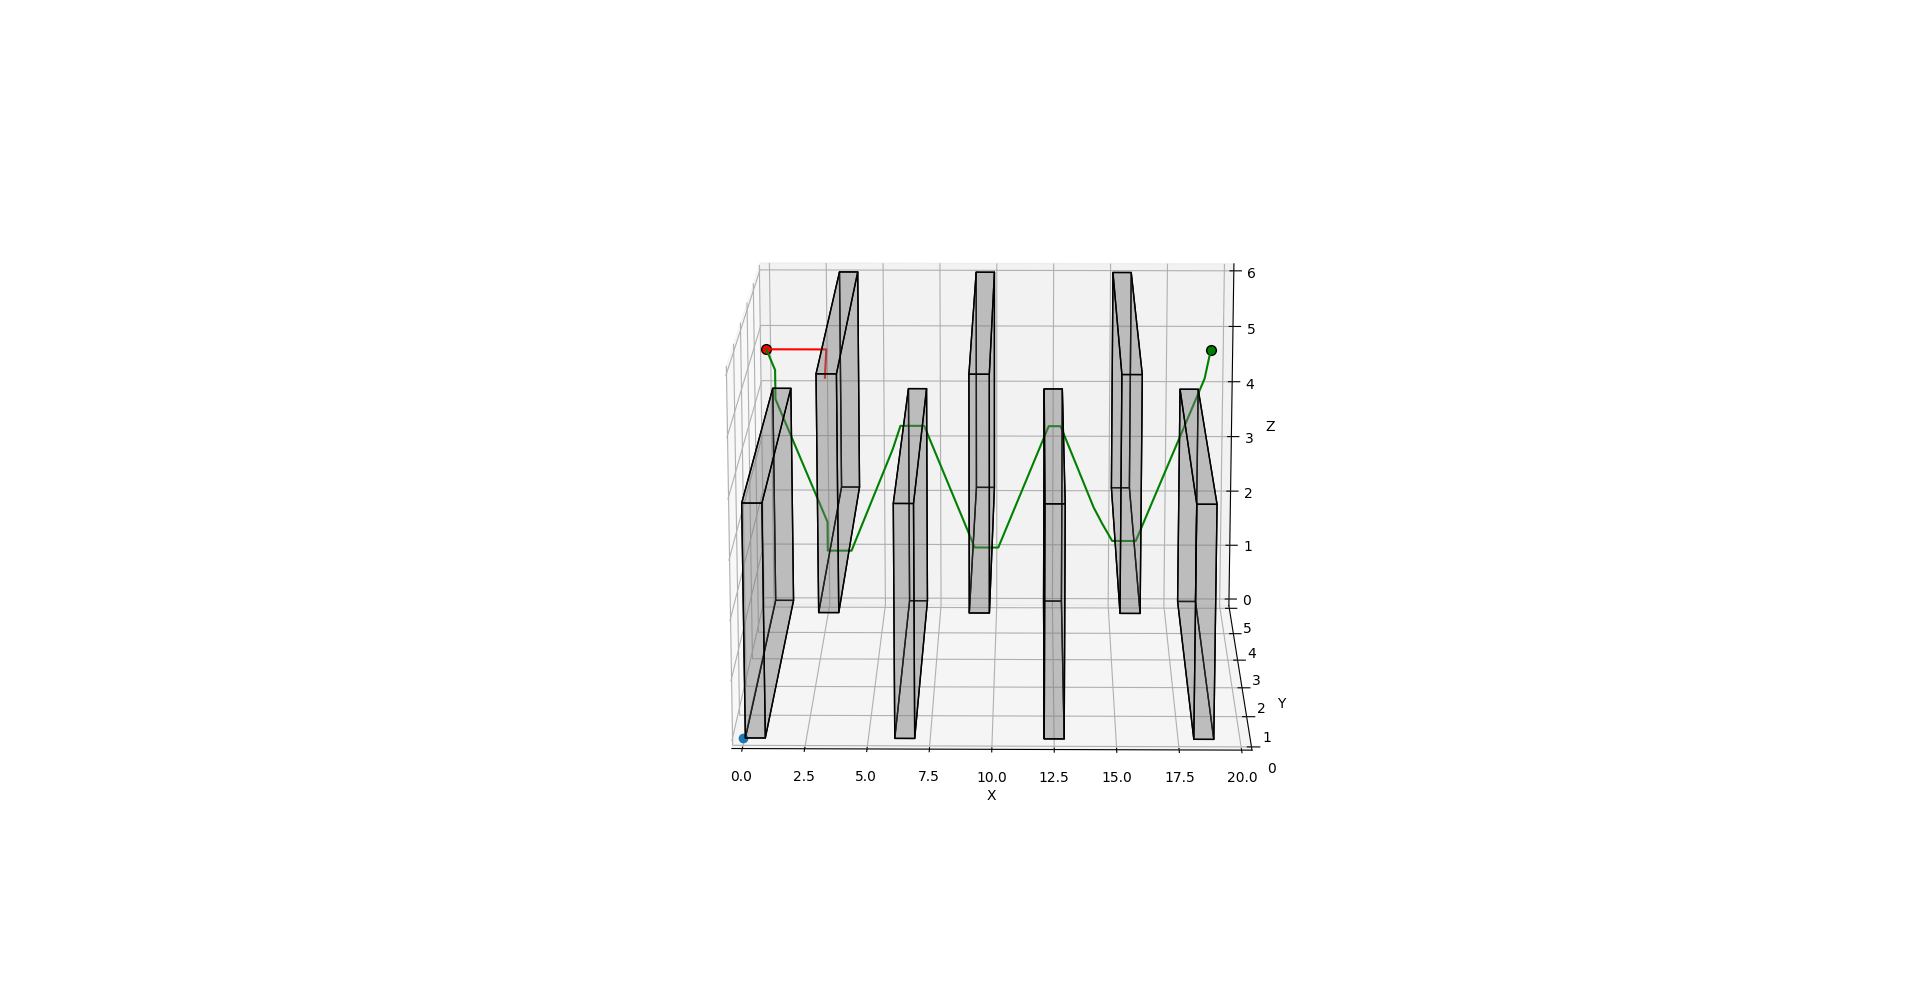
\includegraphics[width=0.5\textwidth]{flappy_bird_astar.png}
    \caption{Path from start (red) to goal (green) in flappy bird environment}
    \label{fig:intro}
\end{figure}
\par RRT is a sampling-based algorithm which is probabilistically complete and asymptotically optimal. It is a tree-based algorithm which grows the tree from the initial state towards the goal state by randomly sampling the state space and connecting the sampled state to the nearest state in the tree.
The distribution for sampling is dependent on the user (uniform or biased towards the goal state). Here we implement the algorithm for uniform, gaussian as well as biased sampling and compare the performance.
The algorithm terminates when the goal state is reached or the tree cannot be expanded further (upto the user to terminate after reaching a particular node count). 
\par A* search is a search-based algorithm which is complete and optimal. It is a graph-based algorithm which grows the graph from the initial state towards the goal state by expanding the node with the lowest cost.
The algorithm terminates when the goal state is reached or the graph cannot be expanded further. The cost of the path is largely dependent on the heuristic function used (designed by the user). Here we implement the algorithm for euclidean, manhattan and chebyshev distance heuristics and compare the performance.
\par As mentioned above both the algorithms are complete and optimal (RRT is asymptotically optimal), the proofs of which will be provided in the following sections.
\section{Problem Formulation}
\label{sec:formulation}
As mentioned above we are trying to solve the DSP problem in a continuous 3D space. Let $\mathcal{B}$ be the space such that
and $\mathcal{B} = \{x \in \mathbb{R}^3 | x_{min} \leq x \leq x_{max}\}$ where $x_{min}$ and $x_{max}$ are the minimum and maximum bounds (opposite vertices of space) of the space (particular environment) respectively.
Similarly, let $\mathcal{O}$ be the set of given obstacles (known environment). 
\begin{itemize}
\item Hence, the state space is $\mathcal{X} = \mathcal{B} \setminus \mathcal{O}$. Let $x_{init}$ and $x_{goal}$ be the initial and goal states respectively. 
\item The control space consists of all the line segments in $\mathcal{X}$. So, $\mathcal{U} = \{(x_i, x_j) \in \mathcal{X} \times \mathcal{X} | x_i \neq x_j\}$. 
\item The cost of the path is the length of the path. So, $c(x_i, x_j) = ||x_i - x_j||_2$ is evaluated same as the heuristic function to keep the heuristic admissible and consistent for convergence of the algorithm. Hence, cost to come will be $g(x_i) = \sum_{j=1}^{i-1} c(x_j, x_{j+1})$ and cost to go will be heuristic function $h(x_i, x_{goal})$.
\item Since, the given state is continuous, we will be using the discretized version of the state space where size of each voxel would be $0.1$ units (discretization is required as we are using a graph-based algorithm).
Now the state space would be corresponding vertex set $\mathcal{V}$ and the edge set (control space) $\mathcal{E}$ would be the set of all the feasible edges between the vertices in $\mathcal{V}$.
\item So, the deterministic shortest path problem is formulated:
\begin{itemize}
    \item Path: sequence $i_{init:q} := (i_{init}, i_1, i_2, \dots, i_q)$ where $i_i \in \mathcal{V}$.
    \item Path length: $g(i_{init}, q) = \sum_{j=1}^{q-1} c(i_j, i_{j+1})$.
    \item All paths from $i_{init}$ to $i_{goal}$: $\mathcal{P} = \{i_{init:q} | i_k \in \mathcal{V}, i_q = i_{goal}\}$.
    \item Objective: find a path which minimizes the following cost function:
    \begin{align*}
        J^* &= \min_{i_{init:q} \in \mathcal{P}} f(i_{init}, q) \\
        i_{init:q}^* &= \operatorname*{arg\,min}_{i_{init:q} \in \mathcal{P}} f(i_{init}, q)
    \end{align*}
    where $f(i_{init}, q)$ is the cost function which is defined seperately for sampling-based and search-based algorithms in the following sections.
\end{itemize}
\end{itemize}

\section{Technical Approach}
To solve the above formulated problem we first have to discretize the state space and implement a collision avoidance algorithms 
to ensure that the nodes generated lie in appropriate configuration space and path obtained would be feasible. In this sections we will
first discuss the collision avoidance algorithm and then the implementation of the two algorithms with various heuristics and sampling distributions.
For the uniformity of the algorithms we have used the same discretization of the state space for both the algorithms. The space is 
discretized with a resolution of 0.1 (this is chosen beacuse in the given environments minimum thickness of the obstacles is 0.1).
\subsection{Collision Avoidance}
Since, the obstacles in the given environments consists only of axis-aligned bounding boxes (AABBs), we will implement a naive approach of finding 
the solution to each of the path segment and obstacle planes. If the solution exists then agent undergoes collision else the path is feasible. In a 3D space,
equation of plane is given by $ax + by + cz + d = 0$ where $(a, b, c)$ is the normal vector to the plane and $(x, y, z)$ is any point on the plane (here $(x,y,z)$ will be constrained depending on the obstacle).
And the equation of line segment between two points $p_1$ and $p_2$ is given by $p = p_1 + t(p_2 - p_1)$ where $t \in [0, 1]$ and $p_i \in \mathcal{X}$. So, substituting the equation of line segment in the equation of plane we get:
\begin{multline*}
    a(p_1 + t(p_2 - p_1)) + b(p_1 + t(p_2 - p_1)) + c(p_1 + t(p_2 - p_1)) + d = 0 \\
    t(a(p_2 - p_1) + b(p_2 - p_1) + c(p_2 - p_1)) + (a + b + c)p_1 + d = 0 \\
    t(a(p_2 - p_1) + b(p_2 - p_1) + c(p_2 - p_1)) = -(a + b + c)p_1 - d \\
    t = \frac{-(a + b + c)p_1 - d}{a(p_2 - p_1) + b(p_2 - p_1) + c(p_2 - p_1)} \\
    t = \frac{-(a + b + c)p_1 - d}{(a + b + c)(p_2 - p_1)}
\end{multline*}
In the above equation if the denominator is zero then the line segment is parallel to the plane and hence no collision. 
If the denominator is non-zero then we have to check if $t \in [0, 1]$ and if it is along with the fact that obtained solution 
lies in the bounding box of the obstacle then the path is in collision. The above procedure is repeated for all the obstacles in the environment.
Above algorithm is not computationally expensive due to the fact that obstacles are AABBs and finite in number (time complexity is $O(n)$ where $n$ is the number of obstacles).
\subsection{Search based Algorithm}
The idea behind search-based algorithms is to generate systematic discretization and search the graph for the optimal path. This is done 
exploring the graph according to a cost function. The completeness and optimality of the algorithm are proved in the lecture slides.
The algorithm is as follows:
\begin{algorithm} \label{alg:alg1}
    \caption{A* Search Algorithm}
\begin{algorithmic}
    \STATE \textbf{function} A*($start, goal, environment$)
    \STATE OPEN $\leftarrow \{start\}$
    \STATE $parent \leftarrow$ an empty map
    \STATE $g \leftarrow$ map with default value $\infty$
    \STATE $g[start] \leftarrow 0$
    \STATE $f \leftarrow$ map with default value $\infty$
    \STATE $f[start] \leftarrow g[start] + h(start, goal)$
    
    \WHILE{$goal \notin$ CLOSED}
        \STATE $current \leftarrow$ node in OPEN with the lowest $f$ value
        \STATE Insert $current$ into CLOSED
        \STATE OPEN $\leftarrow$ OPEN $\setminus \{current\}$
        \FOR{$j \in$ neighbors($current$) and $j \notin$ CLOSED}
            \IF{$g_j > g[current] + c(current, j)$}
                \STATE $parent[j] \leftarrow current$
                \STATE $g[j] \leftarrow g[current] + c(current, j)$
                \STATE $f[j] \leftarrow g[j] + h(j, goal)$
                \IF{$j \in$ OPEN}
                    \STATE Update priority of $j$ in OPEN to $f[j]$
                \ELSE
                    \STATE Insert $j$ into OPEN with priority $f[j]$
                \ENDIF
            \ENDIF
        \ENDFOR
    \ENDWHILE
    \IF{$goal \in$ CLOSED}
        \WHILE{$current \neq start$}
            \STATE Insert $current$ at the beginning of $path$
            \STATE $current \leftarrow parent[current]$
        \ENDWHILE
        \STATE Insert $start$ at the beginning of $path$
        \STATE \textbf{return} $path$
    \ENDIF
    \STATE \textbf{return} failure
    \end{algorithmic}
\end{algorithm} \\
In algorithm \ref{alg:alg1} OPEN list is initialised as a priority queue which consist of candidate nodes for expansion. Map $parent$ gives the relation how nodes are connected (neighbors of a particular node).
$g$ is the cost to come which is defined in \ref{sec:formulation}. $f$ is the total cost of a particular node. $h$ is the heuristic function.
\par The expansion of the nodes is carried according to the priority of the nodes in the OPEN list (determined by $f$). Given that the chosen heuristic is admissible and consistent, the algorithm is complete and optimal (due to the manner in which OPEN list is expanded).
Detailed proof of optimality and completeness is given in lecture slides. More stringent the criterion for admission to OPEN can reduce the number of iterations required by the algorithm. We discuss the behaviour of different heuristics in the next section.
If the path to goal does not exists then the algorithm returns failure. This happens when all possible nodes in the state space is explored and the goal is not found (corollary of completeness).
\par The time and space complexity depends $|\mathcal{V}|$. The time and space complexity of the algorithm is given by $O(|\mathcal{V}|^2)$ and $O(|\mathcal{V}|)$ respectively. The time complexity is due to the fact that we have to iterate over all the nodes in the state space in the worst case scenario.
The space complexity is due to the fact that we have to store all the nodes of the state space in the OPEN list in the worst case scenario.
\par In algorithm \ref{alg:alg1} neighbours are the voxels which are distance ($d$) away from the current voxel in 26 directions (along each edge and vertex of the cube). To make the algorithm efficient in terms of time, we first find the neighbor in continuous state with distance ($d = 0.5$) $\geq$ resolution and later assign the voxel. The cost of moving from one voxel to another is given by the Euclidean distance between the two voxels. The heuristic function is discussed in the next section.
\subsection{Heuristics}
The heuristic function is used to guide the search algorithm towards the goal. The heuristic function is admissible if it never overestimates the cost to reach the goal. 
The heuristic function is consistent if the estimated cost from a node to the goal is less than or equal to the estimated cost from a successor of that node to the goal plus the cost of reaching that successor.
The conditions of optimality and completeness of the algorithm depending upon heuristic is mentioned in lecture slides. We used the following heuristics:
\subsubsection{Euclidean Distance}
The Euclidean distance is the straight line distance between two points. The Euclidean distance is admissible and consistent. The Euclidean distance is given by:
\begin{equation}
    h_{euclidean}(p, q) = ||p - q||_2
\end{equation}
The euclidean distance is admissible as the straight line distance between two points is always less than or equal to the actual cost between the two points (since, $g(x) > 0 \ \forall \ x \in \mathcal{V}$). It also satisfies the triangle inequality and hence is consistent.
So, the path generated by the algorithm with this heuristic is optimal and complete (proved in lecture slides).
\subsubsection{Manhattan Distance}
The Manhattan distance is the distance between two points measured along axes at right angles. Since, expansion of neighbours is also carried out along the diagonal direction, the Manhattan distance is neither admissible nor consistent. The Manhattan distance is given by:
\begin{equation}
    h_{manhattan}(p, q) = ||p - q||_1
\end{equation}
Since, the manhattan distance is an inadmissible but $\epsilon$-consistent heuristic, the path generated by the algorithm would be $\epsilon$-suboptimal ($\forall \ \epsilon \geq 1$). To make the algorithm complete
we would have to re-open the closed nodes. The results are discussed in the following section.
\subsubsection{Chebychev Distance}
The Chebychev distance is the maximum of the absolute difference between the two points. The Chebychev distance is admissible as it calculates the maximum absolute difference between x, y, and z coordinates. The Chebychev distance is given by:
\begin{equation}
    h_{chebychev}(p, q) = \max(|p_x - q_x|, |p_y - q_y|, |p_z - q_z|)
\end{equation}
Since, above heuristic is admissible and consistent the path generated by the algorithm is optimal and algorithm is complete. The results are discussed in the following section.
\subsubsection{Octile Distance}
The octile distance is given by:
\begin{multline*}
h_{octile}(p, q) = \max(|p_x - q_x|, |p_y - q_y|, |p_z - q_z|) \\
+ (\sqrt{3} - 1) \min(|p_x - q_x|, |p_y - q_y|, |p_z - q_z|)
\end{multline*}
In a 3D environment, the Octile Distance heuristic can be considered admissible (corollary of problem 2 in Homework 2). It provides a lower bound on the actual cost to reach the goal from a given state, as it considers both the horizontal/vertical cost and the diagonal cost. 
Therefore, it will not overestimate the cost and remains admissible. The Octile distance heuristic is also consistent. Hence, path genrated would be optimal and algorithm is complete. The results are discussed in the following section.
\subsection{Sampling-Based Algorithm}
The sampling-based algorithm generates a graph by randomly sampling nodes in the state space and connecting them to the nearest neighbours. It searches the graph for a path, guaranteeing that the probability of finding one if 
it exists approches 1 as the number of samples approaches infinity. It provides asymptotic suboptimality bounds on the solution. The samples are generated only when necessary. Depending upon the environment it can be faster
and memory efficient than search-based algorithm.
\par Here, we are implementing Rapidly-exploring Random Tree (RRT) algorithm. The algorithm is given in Algorithm \ref{alg:alg2}. The algorithm is initialized with the start node. A tree is constructed from random samples 
in the state space. It is expanded until it contains path to the goal (within a certain threshold).
\begin{algorithm}
\caption{Rapidly-exploring Random Tree (RRT)}
\label{alg:alg2}
\begin{algorithmic}
\STATE $V \gets \{x_{init}\}; E \gets \emptyset$
\FOR{$k = 1$ to $K$}
\STATE $x_{rand} \gets$ Sample()
\STATE $x_{nearest} \gets$ Nearest($(T, E), x_{rand}$)
\STATE $x_{new} \gets$ Steer($x_{nearest}, x_{rand}, \epsilon$)
\IF{ObstacleFree($x_{nearest}, x_{new}$)}
\STATE $T \gets T \cup \{x_{new}\}$ ; $E \gets E \cup \{(x_{nearest}, x_{new})\}$
\IF{$||x_{new} - x_{goal}||_2 <$ threshold}
\STATE $G = (T, E)$
\STATE break
\ENDIF
\ENDIF
\ENDFOR
\IF {$x_{goal} \notin T$}
\STATE \textbf{return} Failure
\ENDIF
\STATE path $\gets$ \{$x_{goal}$\}; $x_{current} \gets x_{goal}$
\WHILE{$x_{current} \neq x_{init}$}
\STATE $x_{parent} \gets$ Parent($x_{current}$)
\STATE path $\gets$ path $\cup$ \{$x_{parent}$\}
\STATE $x_{current} \gets x_{parent}$
\ENDWHILE
\STATE \textbf{return} path
\end{algorithmic}
\end{algorithm}
\par In the Algorithm \ref{alg:alg2}, the function Sample() returns a random sample (we tested various sampling distributions which are discussed in the Results) from the state space. We can minimize the cost mentioned in \ref{sec:formulation} by choosing appropriate sampling strategy. For instance, we could sample with a bias towards which could help us minimize the cost. The function Nearest() returns the nearest node in the tree to the random sample. The function Steer() returns a node
that is at most $\epsilon$ distance away from the nearest node in the direction of the random sample. Since, our agent does not have any dynamics we can extract the new node ($x_{new}$) by simple extrapolation. If $x_{new}$ is in collision with any obstacle, the node is discarded in our implementation (we could have extended the tree upto the obstacle boundary).
The function ObstacleFree() returns true if the path between the two nodes is free of obstacles which is same collision avoidance function 
as used for search-based algorithm. 
\par If the algorithm could not find the path within given number of iterations, we might have to increase the number of iterations or increase the threshold distance. 
For the algorithm to converge faster we can increase the $\epsilon$ so that the tree is expanded faster in terms of distance. We can also conduct sampling which is biased towards the goal node to converge faster.
The algorithm returns the path from the goal node to the start node. The path is obtained by backtracking from the goal node to the start node.
\section{Results and Discussion}
For the sake of uniformity we will be considering the pathlength as sum of Euclidean distance between the nodes which form the extracted path.
This is done so that we can quantitatively evaluate the optimality of the algorithms.
\subsection{Search-Based Algorithm}
\begin{table}[h]
    \centering
    \caption{Search-Based Algorithm Euclidean heuristic}
    \label{tab:tab1}
    \begin{tabular}{|c|c|c|c|}
    \hline
    & \textbf{Time(s)} & \textbf{Path Length} & \textbf{No. of Nodes Expanded} \\ \hline
    \textbf{Single Cube} & 0.0945 & 8.14 & 156 \\ \hline
    \textbf{Maze} & 5543.542 & 74.155 & 1054569 \\ \hline
    \textbf{Flappy Bird} & 619.72 & 25.66 & 263839 \\ \hline
    \textbf{Monza} & 304.49 & 75.66 & 292230 \\ \hline
    \textbf{Window} & 729.27 & 26.3 & 275272 \\ \hline
    \textbf{Tower} & 1330.94 & 28.12 & 194940 \\ \hline
    \textbf{Room} & 62.42 & 11.16 & 9635 \\ \hline
    \end{tabular}
    \end{table}
The results are mentioned in Table \ref{tab:tab1}, \ref{tab:tab2}, \ref{tab:tab3} and \ref{tab:tab4}. Analysis for the search-based algorithm is mentioned below:
\begin{itemize}
    \item The algorithm is able to find the path for all the environments. We also observed that the path generated is optimal using all the mentioned heuristics. 
    \item Although the path generated are optimal using different heuristics, the number of nodes visited are quite different. Also the runtime of the algorithm is different for different heuristics (quite large difference in some cases). This is because the algorithm 
    added bunch of useless nodes to the open list as a result of quality of the heuriatic function.
    \item We can conclude that the lagorithm using euclidean heuristic is optimal in terms of time complexity (expands least number or almost least of nodes in each environment).
    Despite the fact mentioned above heuristic different from Euclidean distance gave exceedingly better results in some environments.
    \item Since, A* star algorithm expands it search layerwise it takes lot of time to find path in environments with large number of obstacles (like maze) and depending on the positioning of the start and goal. Such as in maze environment, start node is in the center of the 
    maze and goal node is in the corner of the maze. In such cases, the algorithm expands the nodes in the maze and takes lot of time to find the path.
\end{itemize}
\begin{table}[h]
    \centering
    \caption{Search-Based Algorithm Chebychev heuristic}
    \label{tab:tab2}
    \begin{tabular}{|c|c|c|c|}
    \hline
    & \textbf{Time(s)} & \textbf{Path Length} & \textbf{No. of Nodes Expanded} \\ \hline
    \textbf{Single Cube} & 28.9 & 8.14 & 103912 \\ \hline
    \textbf{Maze} & 6872 & 74.55 & 1554569 \\ \hline
    \textbf{Flappy Bird} & 756.26 & 25.7 & 417515 \\ \hline
    \textbf{Monza} & 354.64 & 75.69 & 385478 \\ \hline
    \textbf{Window} & 1214.15 & 26.16 & 643533 \\ \hline
    \textbf{Tower} & 1470.72 & 27.98 & 320149 \\ \hline
    \textbf{Room} & 290.97 & 11.16 & 82334 \\ \hline
    \end{tabular}
\end{table}
Hence, choosing appropriate heuristic function is very important for the search-based algorithm depending on the environment and motion model of the agent as it could improve the performance of the algorithm significantly. Since, paths with different heuristics
could have different strains on the controller of the agent. This could be also be kept in mind while choosing the heuristic (which does not involve extremely sharp turns or sudden changes in velocity).
Since, nodes are explored in a systematic manner, so we would always obtain (almost) same path for same environemt given heuristic is also same.
We did not plot all the explored as it would make the graph really cluttered for analysis. To plot this please go through README.md provided with the script.
\begin{table}[h]
    \centering
    \caption{Search-Based Algorithm Manhattan heuristic}
    \label{tab:tab3}
    \begin{tabular}{|c|c|c|c|}
    \hline
    & \textbf{Time(s)} & \textbf{Path Length} & \textbf{No. of Nodes Expanded} \\ \hline
    \textbf{Single Cube} & 0.012 & 8.14 & 398 \\ \hline
    \textbf{Maze} & 5113.23 & 74.40 & 1140113 \\ \hline
    \textbf{Flappy Bird} & 478.19 & 25.9 & 301219 \\ \hline
    \textbf{Monza} & 259.504 & 76.2 & 295583 \\ \hline
    \textbf{Window} & 1377 & 26.3 & 326293 \\ \hline
    \textbf{Tower} & 1167.58 & 29 & 259492 \\ \hline
    \textbf{Room} & 37.54 & 11.65 & 13791 \\ \hline
    \end{tabular}
\end{table}
\begin{table}[h]
    \centering
    \caption{Search-Based Algorithm Octile heuristic}
    \label{tab:tab4}
    \begin{tabular}{|c|c|c|c|}
    \hline
    & \textbf{Time(s)} & \textbf{Path Length} & \textbf{No. of Nodes Expanded} \\ \hline
    \textbf{Single Cube} & 0.15 & 8.14 & 3642 \\ \hline
    \textbf{Maze} & 7844.13 & 74.55 & 2067456 \\ \hline %do for all
    \textbf{Flappy Bird} & 669.45 & 25.6 & 386774 \\ \hline
    \textbf{Monza} & 404.9 & 75.5 & 380320 \\ \hline
    \textbf{Window} & 675.79 & 26.3 & 439646 \\ \hline
    \textbf{Tower} & 1502.82 & 28.8 & 309182 \\ \hline %do
    \textbf{Room} & 390.46 & 11.16 & 18861 \\ \hline %do
    \end{tabular}
\end{table}
\subsection{Sampling-Based Algorithm}
\begin{table}
    \centering
    \caption{Sampling-Based Algorithm Uniform distribution}
    \label{tab:tab5}
    \begin{tabular}{|c|c|c|c|}
    \hline
    & \textbf{Time(s)} & \textbf{Path Length} & \textbf{No. of Nodes Expanded} \\ \hline
    \textbf{Single Cube} & 5.62 & 15.84 & 2709 \\ \hline
    \textbf{Maze} & 770.591 & 128 & 17362 \\ \hline
    \textbf{Flappy Bird} & 4.03 & 43.06 & 1965 \\ \hline
    \textbf{Monza} & 1491.26 & 113.66 & 30754 \\ \hline
    \textbf{Window} & 0.2 & 30.59 & 384 \\ \hline
    \textbf{Tower} & 6.79 & 41.25 & 1885 \\ \hline
    \textbf{Room} & 0.66 & 13.13 & 628 \\ \hline
    \end{tabular}
    \end{table}
The results are mentioned in Table \ref{tab:tab5} and \ref{tab:tab6} (probability of sampling of goal is chosen as 0.4). The threshold of reaching goal is set as 0.5 units. Analysis for the sampling-based algorithm is mentioned below:
\begin{itemize}
    \item The algorithm is able to find the path for all the environments given the number of iterations is sufficiently large. Although the path generated is far from optimal several times mainly in open environments. This is due to the fact that we are sampling from a uniform distribution. 
    This shortcoming could be overcome by using a biased sampling distribution.
    \item The algorithm is extremely fast for cluttered environments as we are directly sampling from the state space and not expanding the tree layerwise. So, when most of space is covered with obstacles
    the algorithm samples the nodes free space (the size of which is reduced) and hence the algorithm converges faster. Although, if the goal node is covered by obstacle with small opening (concave obstacle) the algorithm could be slower as seen the case of window environment.
    \item The number of nodes expanded is also dependent on the sampling distribution. If we use a biased sampling distribution which is biased towards the goal node, the algorithm will converge faster and sample less number of nodes (depends on the bias of the distribution).
    \item We can obtain the optimal path by increasing the number of nodes to be sampled and changing the termination condition of the algorithm. But, this will significantly increase the time taken by the algorithm.
    \item We observed that this is the case only when environment is relatively open. If the environment is cluttered, the algorithm will converge faster if we use a uniform sampling distribution.
    So, depending upon the environment we should choose the sampling distribution and use this algorithm. Since, the nodes are generated by sampling we won't always get the same path for the same environment.
\end{itemize}
\begin{table}
    \centering
    \caption{Sampling-Based Algorithm Biased distribution}
    \label{tab:tab6}
    \begin{tabular}{|c|c|c|c|}
    \hline
    & \textbf{Time(s)} & \textbf{Path Length} & \textbf{No. of Nodes Expanded} \\ \hline
    \textbf{Single Cube} & 0.04 & 12.28 & 159 \\ \hline
    \textbf{Maze} & 756.961 & 120.68 & 15166 \\ \hline 
    \textbf{Flappy Bird} & 7.54 & 42.7 & 2469 \\ \hline
    \textbf{Monza} & 1259.47 & 118.66 & 25532 \\ \hline %do
    \textbf{Window} & 7.85 & 39.39 & 2973 \\ \hline
    \textbf{Tower} & 2.24 & 39.92 & 1154 \\ \hline
    \textbf{Room} & 0.42 & 25.07 & 427 \\ \hline
    \end{tabular}
    \end{table}
\subsection{Comparison}
From the above discussion we conclude that depending on the heuristic function A* guarantees optimality and completeness whereas RRT is probabilistically complete.
\par The search-based algorithm is able to find the optimal path in all the environments. But it is extremely slow in cluttered environments. Whereas the sampling-based algorithm is extremely fast in cluttered environments but it is not able to find the optimal path in open environments. And the path found is also quite noisy.
\par So, depending on the environment we can choose the algorithm. If the environment is cluttered we can use sampling-based algorithm and if the environment is open we can use search-based algorithm. But if the environment contains really narrow passages, the discussed sampling based algorithm might have hard time finding the path within reasonable time. In such cases we might have to make certain modifications to the algorithm like RRT* or bi-directional RRT.
\par The A* algorithm can still be improved by employing multiple resolution in the search space. This will help in reducing the number of nodes expanded and hence the time taken to find the path. We can use higher resolution near the obstacles and lower resolution in the free space. This will help in reducing the number of nodes expanded and hence the time taken to find the path.
\par The RRT algorithm can be improved by using a biased sampling distribution. This will help in converging faster. We can also use RRT* or bi-directional RRT to improve the algorithm.
\par One key difference, is that A* would always generate same path for the same environment (given the heuristic is same). Whereas, RRT would generate different paths for the same environment. This is because RRT is a sampling-based algorithm and the nodes are generated by sampling. So, we won't always get the same path for the same environment.
\section{Plots}
Since, there was not much difference in the trajectories of the path for different heuristics, we only show the plots for the Euclidean and Manhattan heuristic.
Red path is the one generated by baseline planner.
\subsection{A* Euclidean Heuristic}
A* planned path shown in green. Red path is the one generated by baseline planner.
\begin{figure}[H]
    \centering
    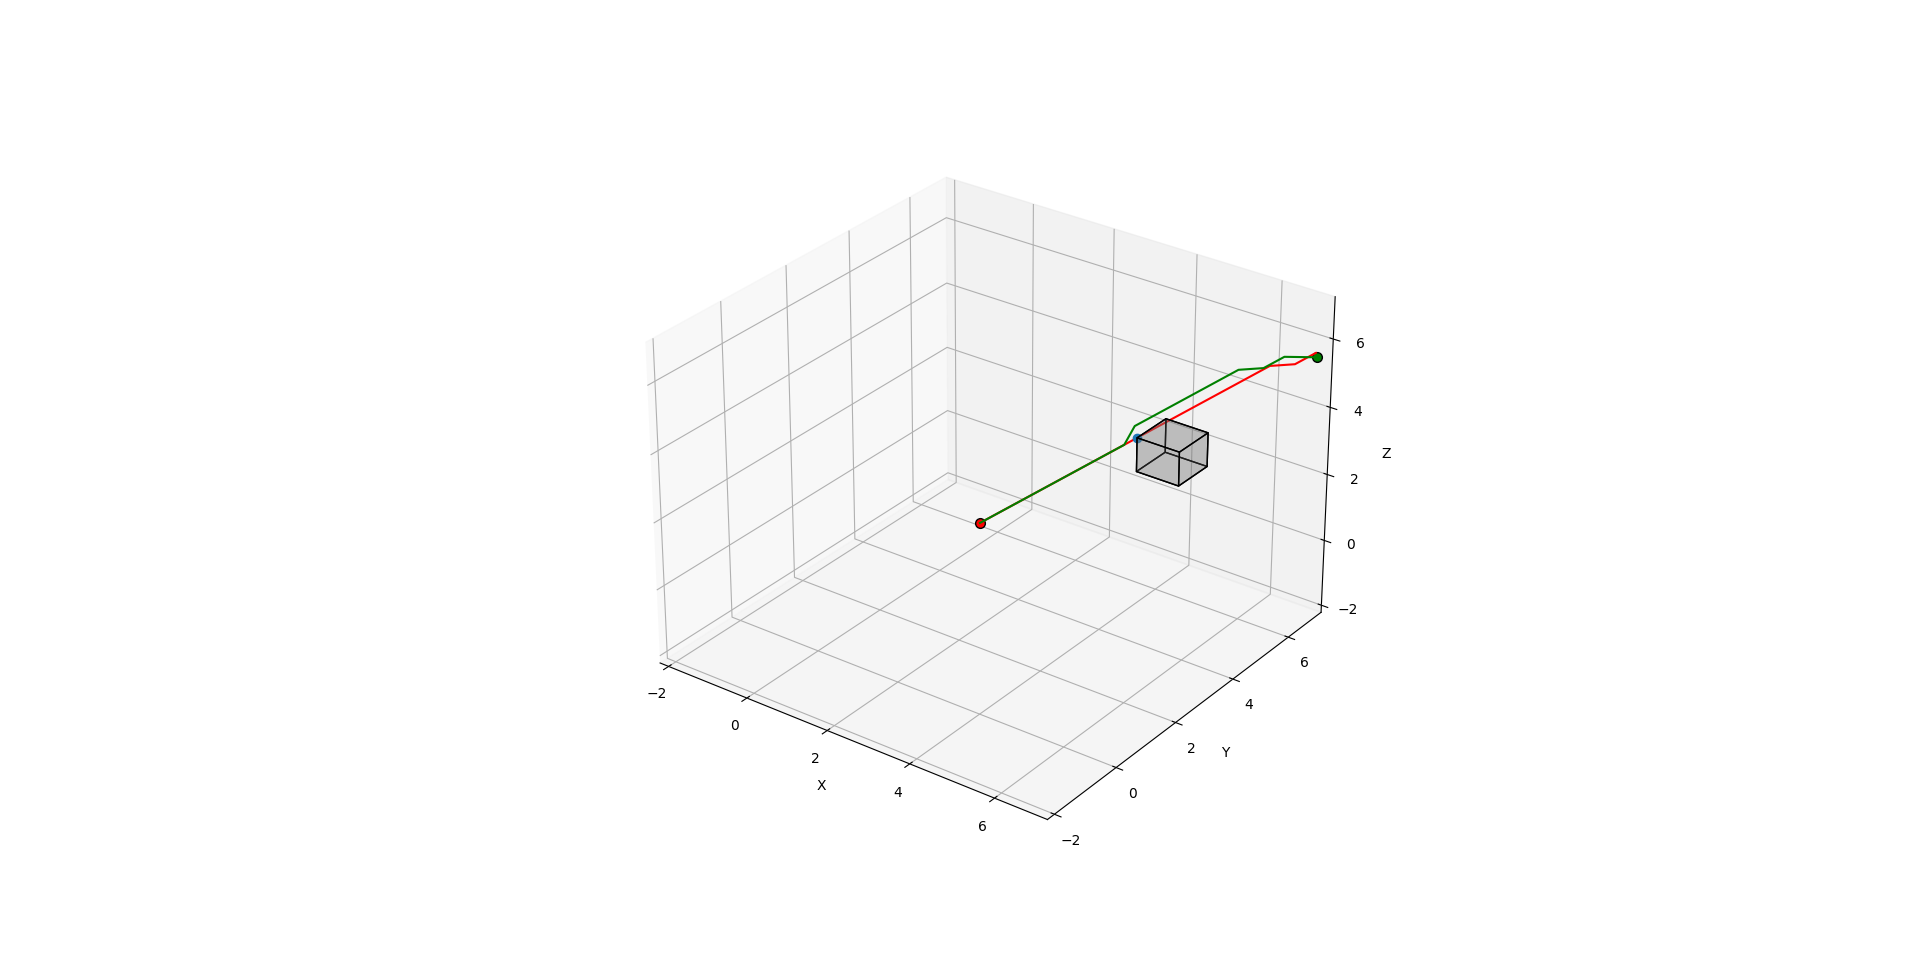
\includegraphics[width=0.6\textwidth]{cube_astar.png}
    \caption{Single Cube Environment}
    \label{fig:cube_astar}
\end{figure}
\begin{figure}[H]
    \centering
    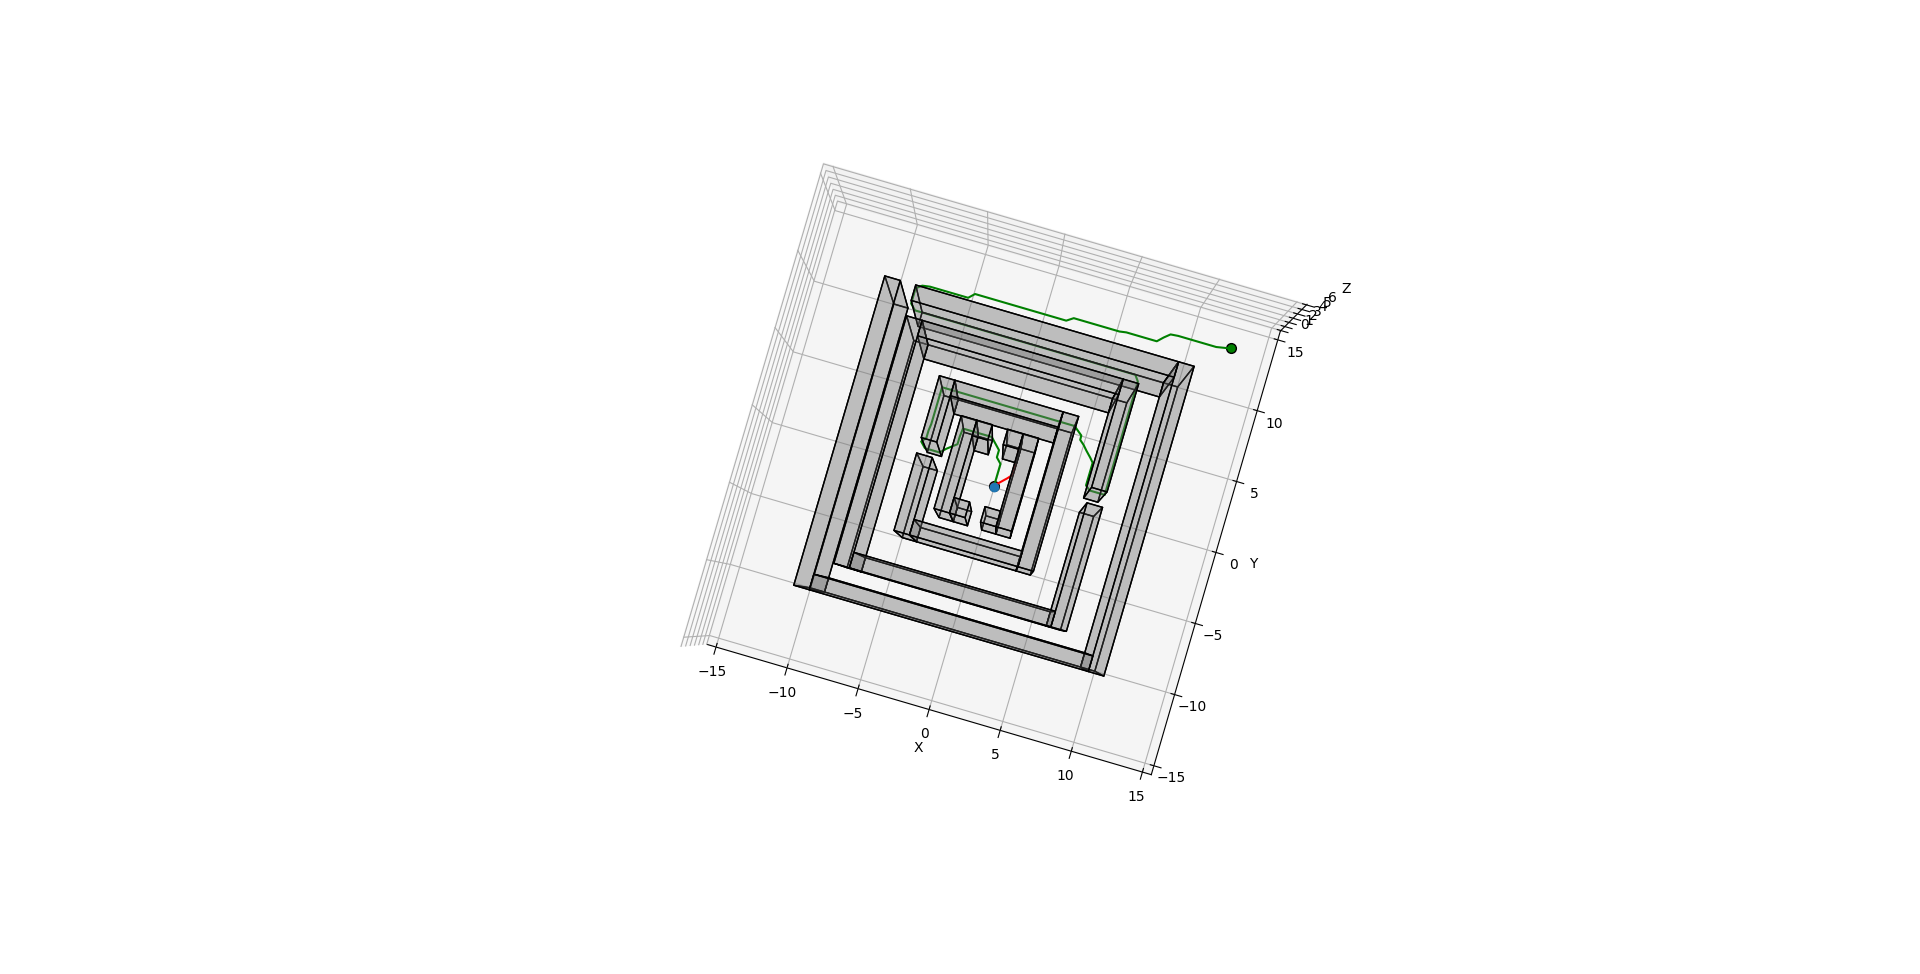
\includegraphics[width=0.6\textwidth]{maze_astar.png}
    \caption{Maze Environment}
    \label{fig:maze_astar}
\end{figure}
\begin{figure}[H]
    \centering
    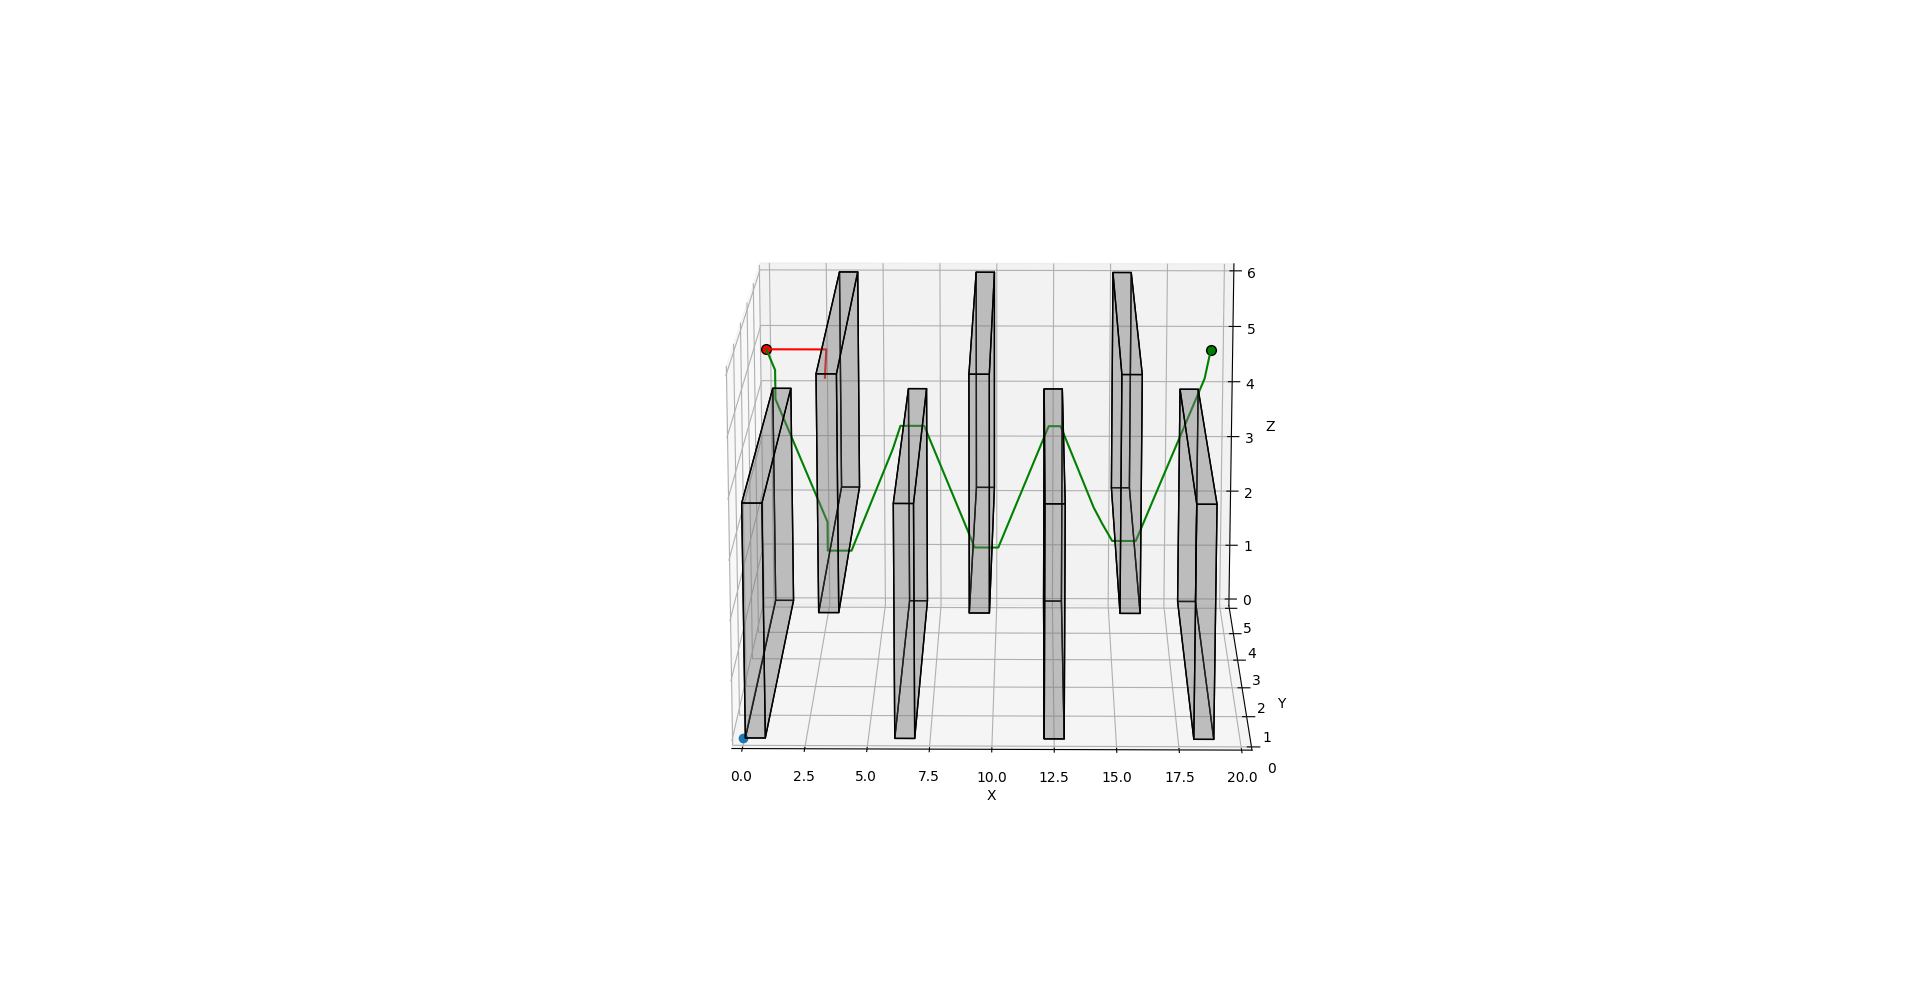
\includegraphics[width=0.6\textwidth]{flappy_bird_astar.png}
    \caption{Flappy Bird Environment}
    \label{fig:flappy_bird_astar}
\end{figure}
\begin{figure}[H]
    \centering
    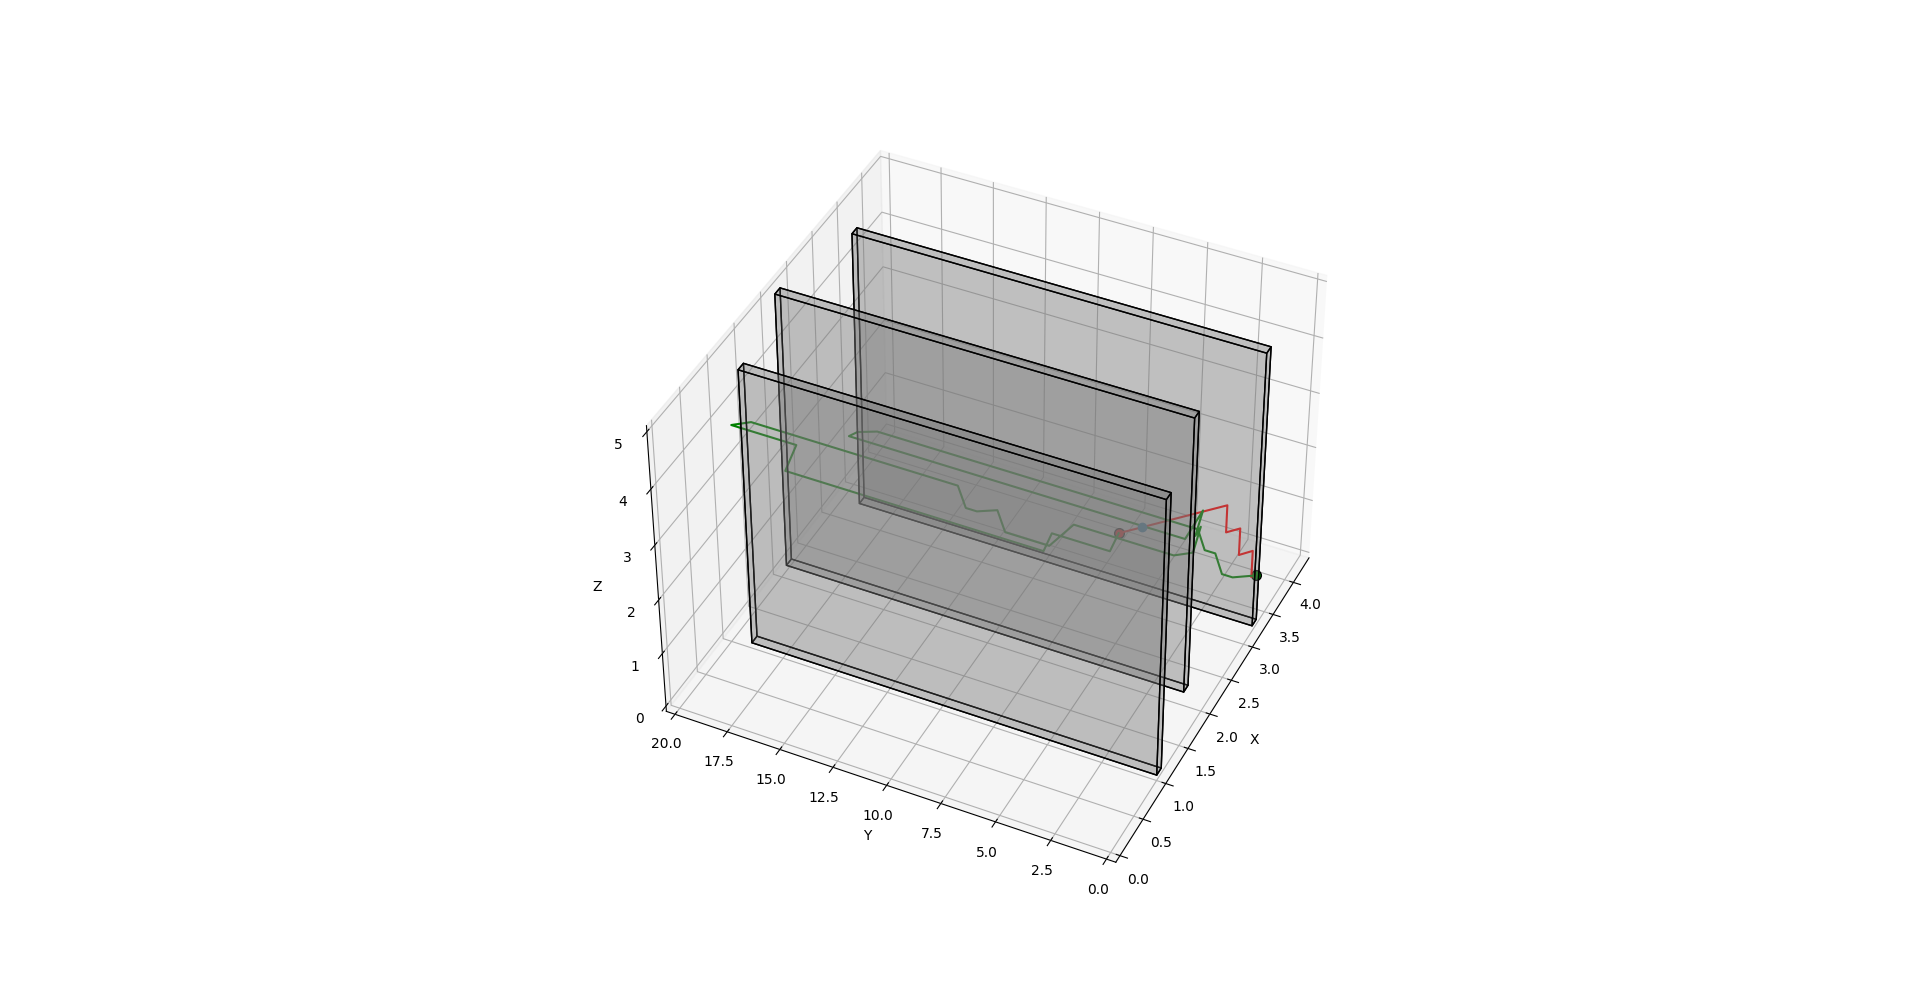
\includegraphics[width=0.6\textwidth]{monza_astar.png}
    \caption{Monza Environment}
    \label{fig:monza_astar}
\end{figure}
\begin{figure}[H]
    \centering
    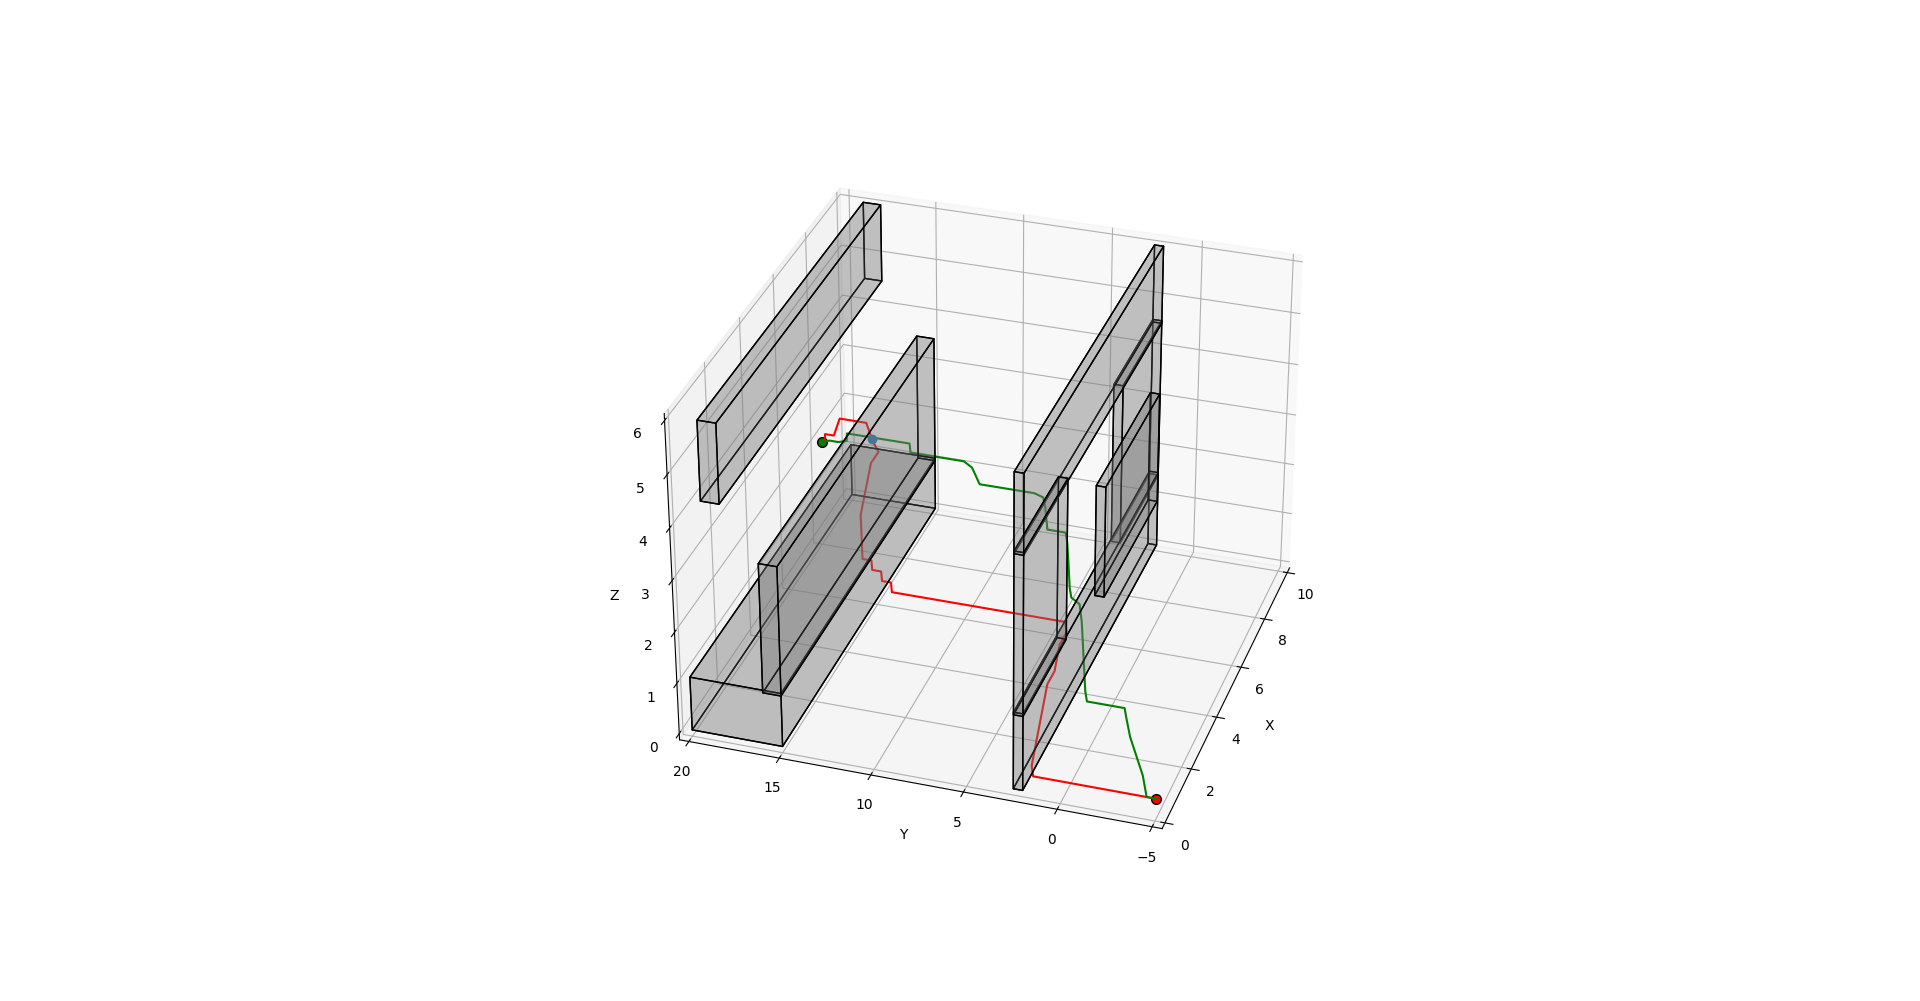
\includegraphics[width=0.6\textwidth]{window_astar.png}
    \caption{Window Environment}
    \label{fig:window_astar}
\end{figure}
\begin{figure}[H]
    \centering
    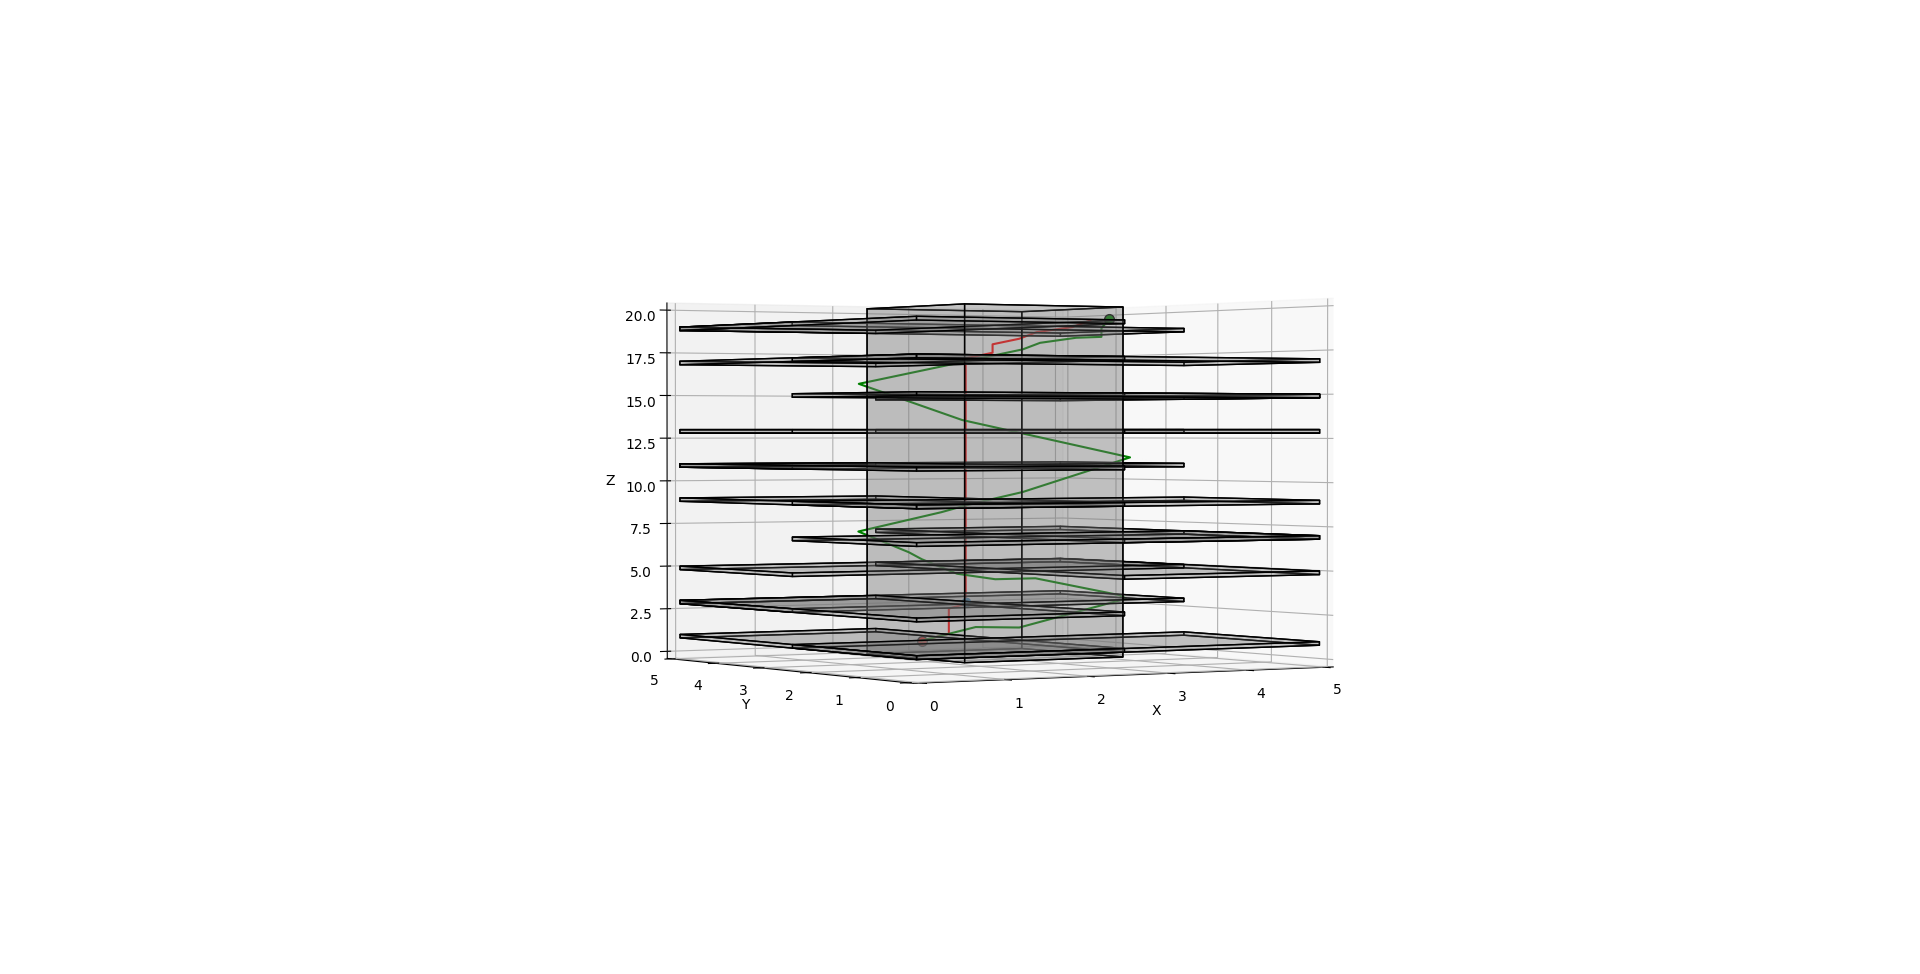
\includegraphics[width=0.6\textwidth]{tower_astar.png}
    \caption{Tower Environment}
    \label{fig:tower_astar}
\end{figure}
\begin{figure}[H]
    \centering
    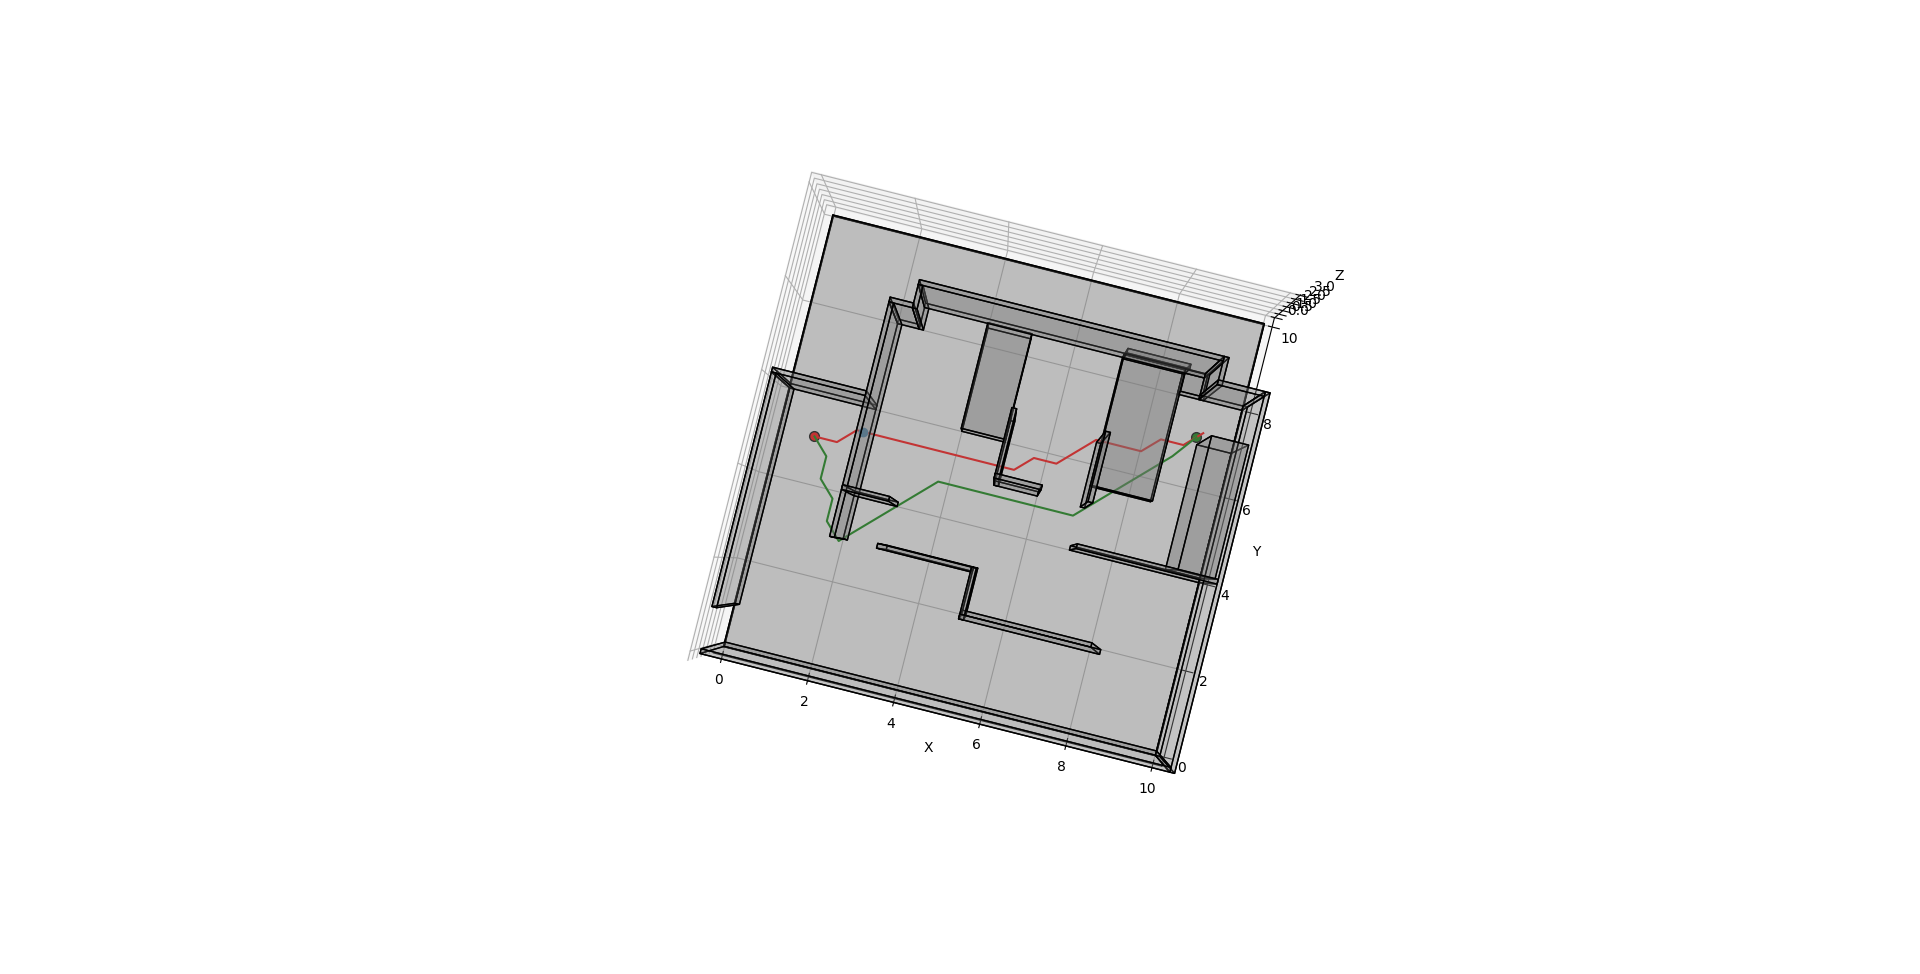
\includegraphics[width=0.6\textwidth]{room_astar.png}
    \caption{Room Environment}
    \label{fig:room_astar}
\end{figure}
\subsection{A* Manhattan Heuristic}
\begin{figure}[H]
    \centering
    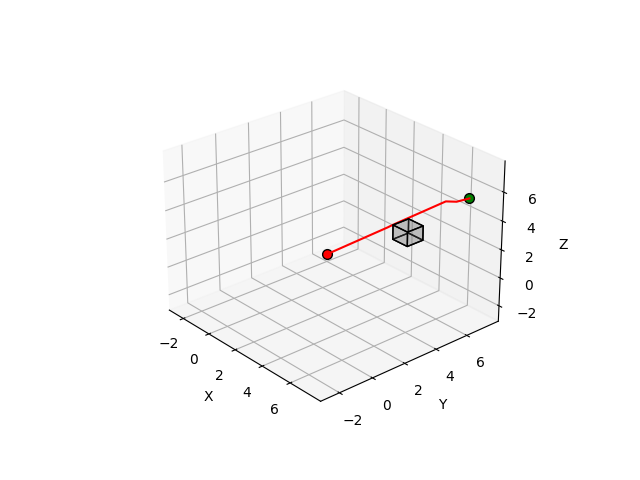
\includegraphics[width=0.6\textwidth]{cube_astar_m.png}
    \caption{Single Cube Environment}
    \label{fig:cube_astar_m}
\end{figure}
\begin{figure}[H]
    \centering
    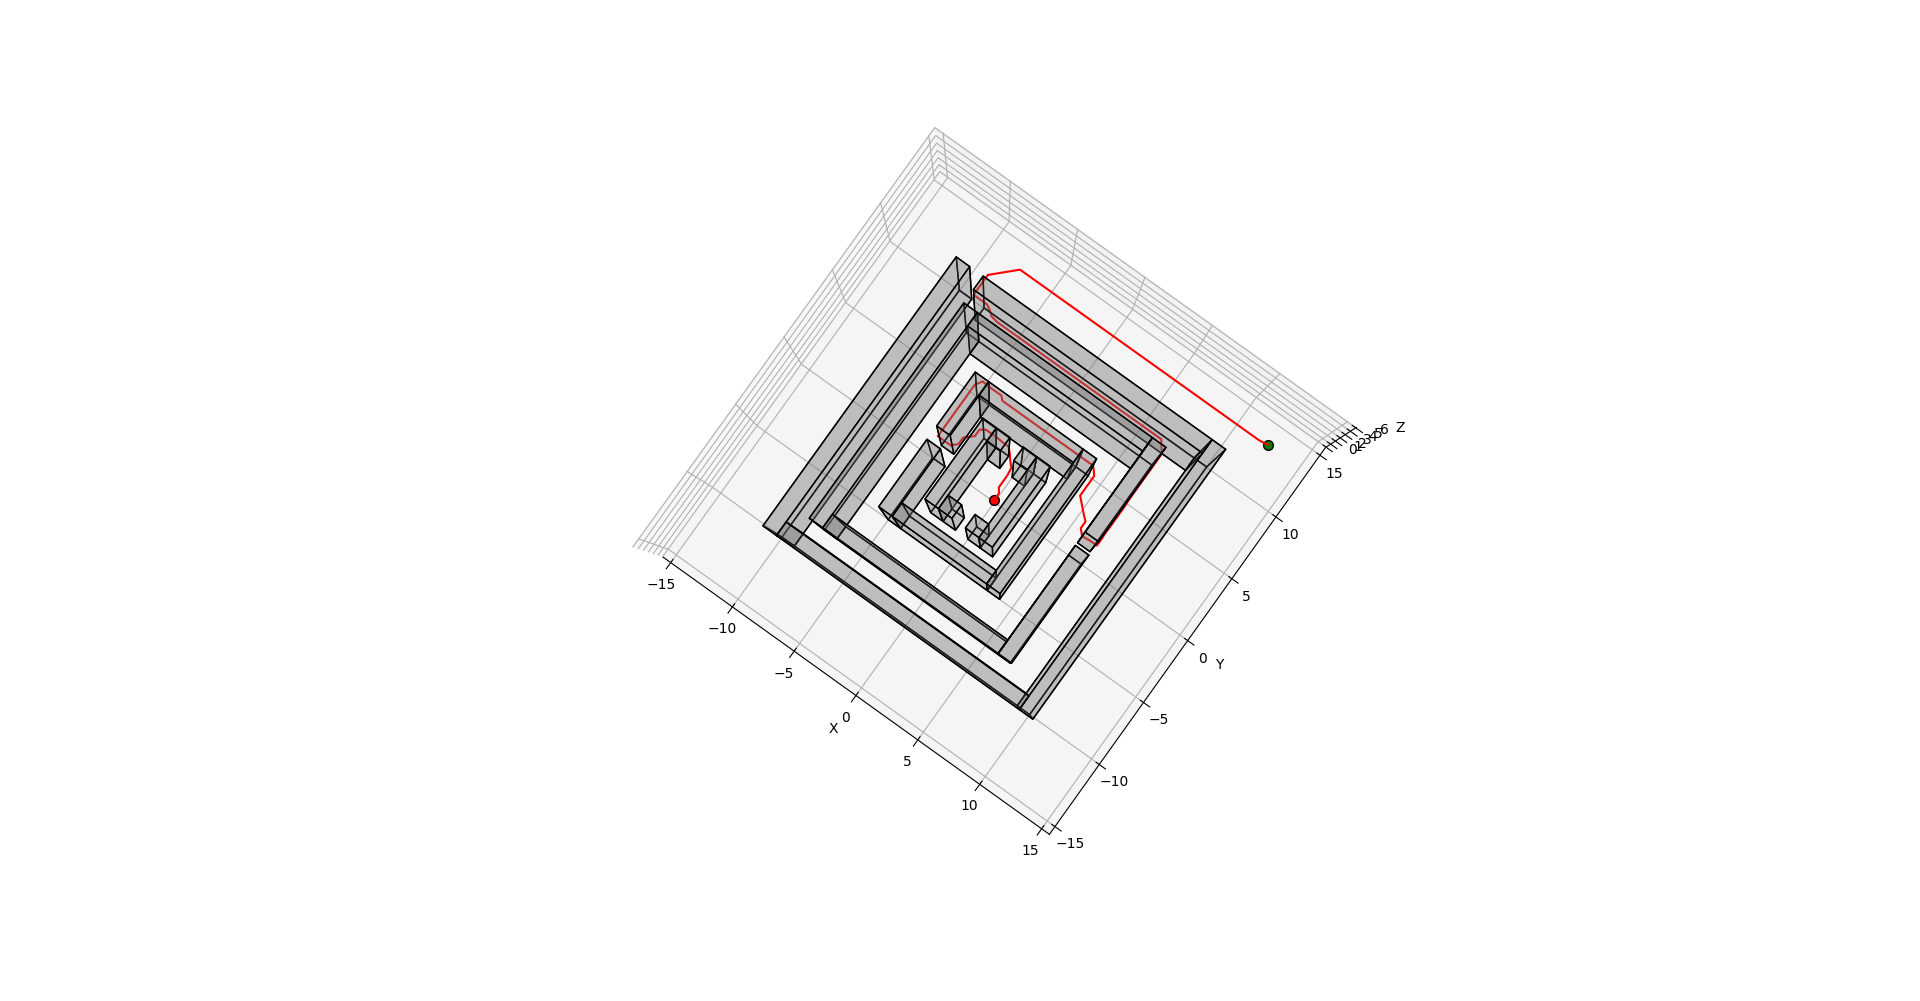
\includegraphics[width=0.6\textwidth]{maze_astar_m.png}
    \caption{Maze Environment}
    \label{fig:maze_astar_m}
\end{figure}
\begin{figure}[H]
    \centering
    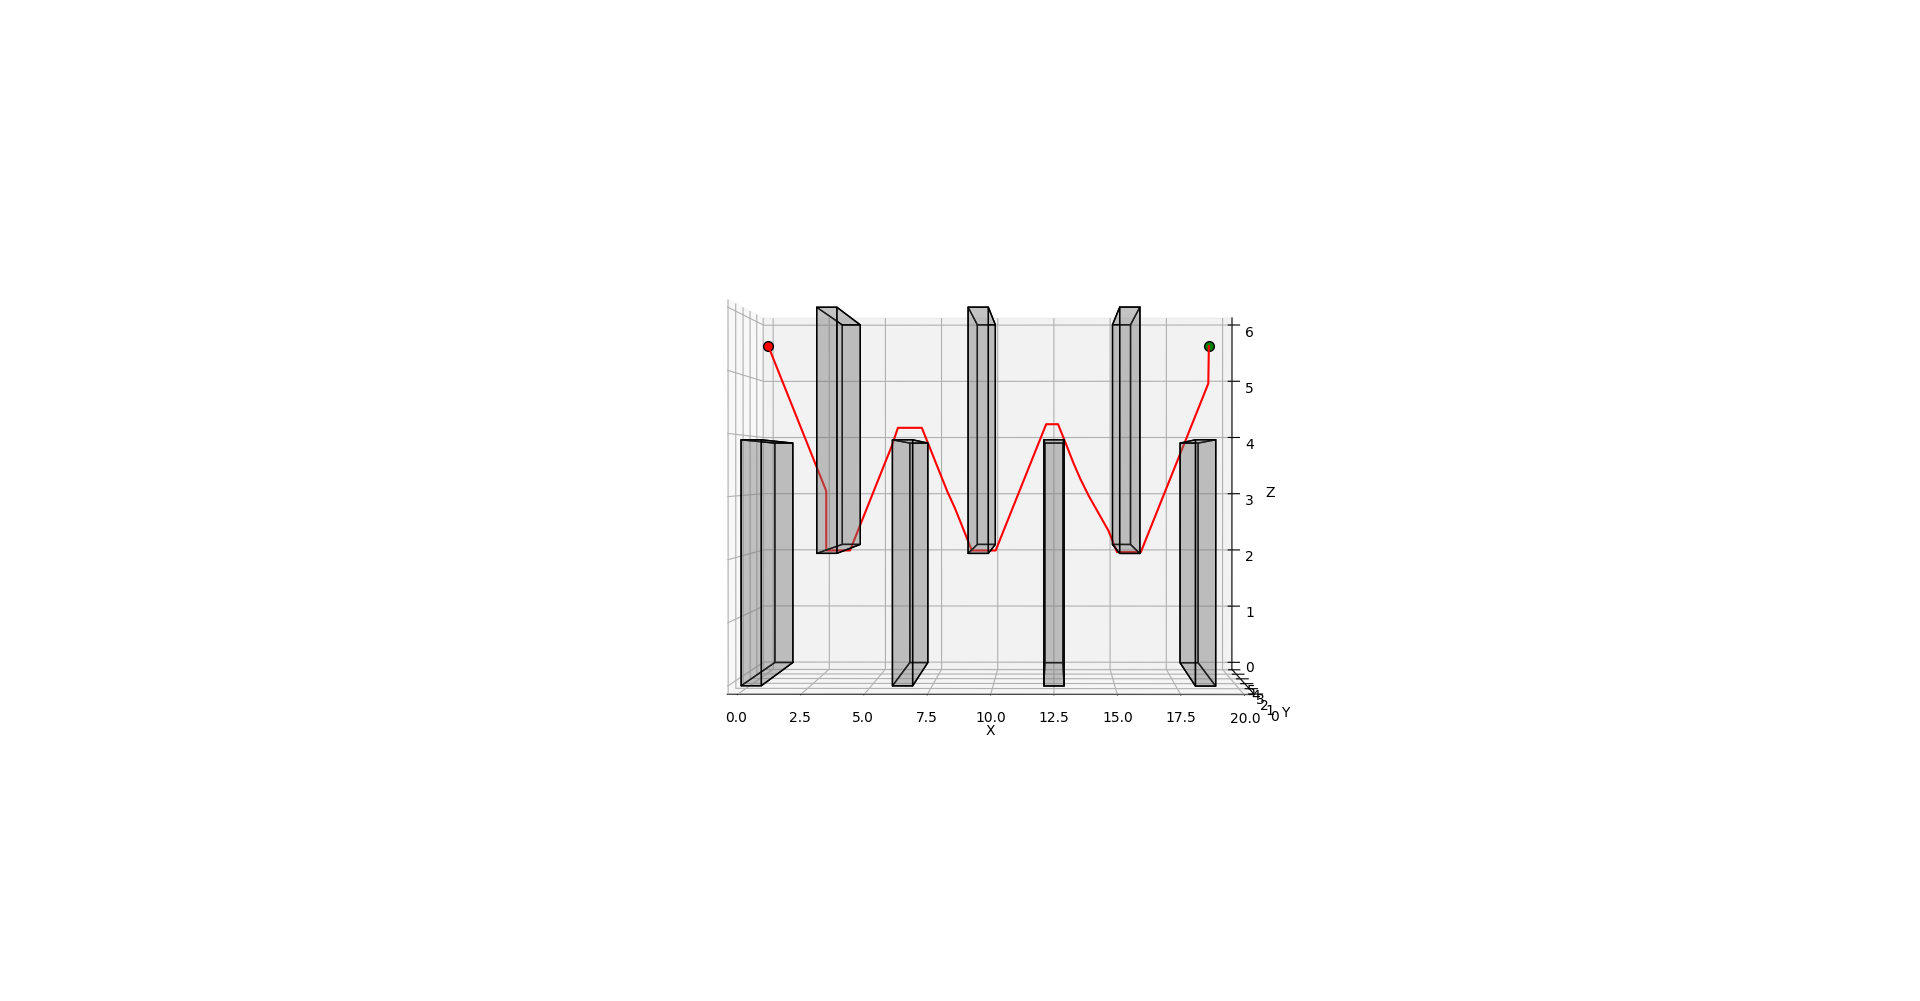
\includegraphics[width=0.6\textwidth]{flappy_bird_astar_m.png}
    \caption{Flappy Bird Environment}
    \label{fig:flappy_bird_astar_m}
\end{figure}
\begin{figure}[H]
    \centering
    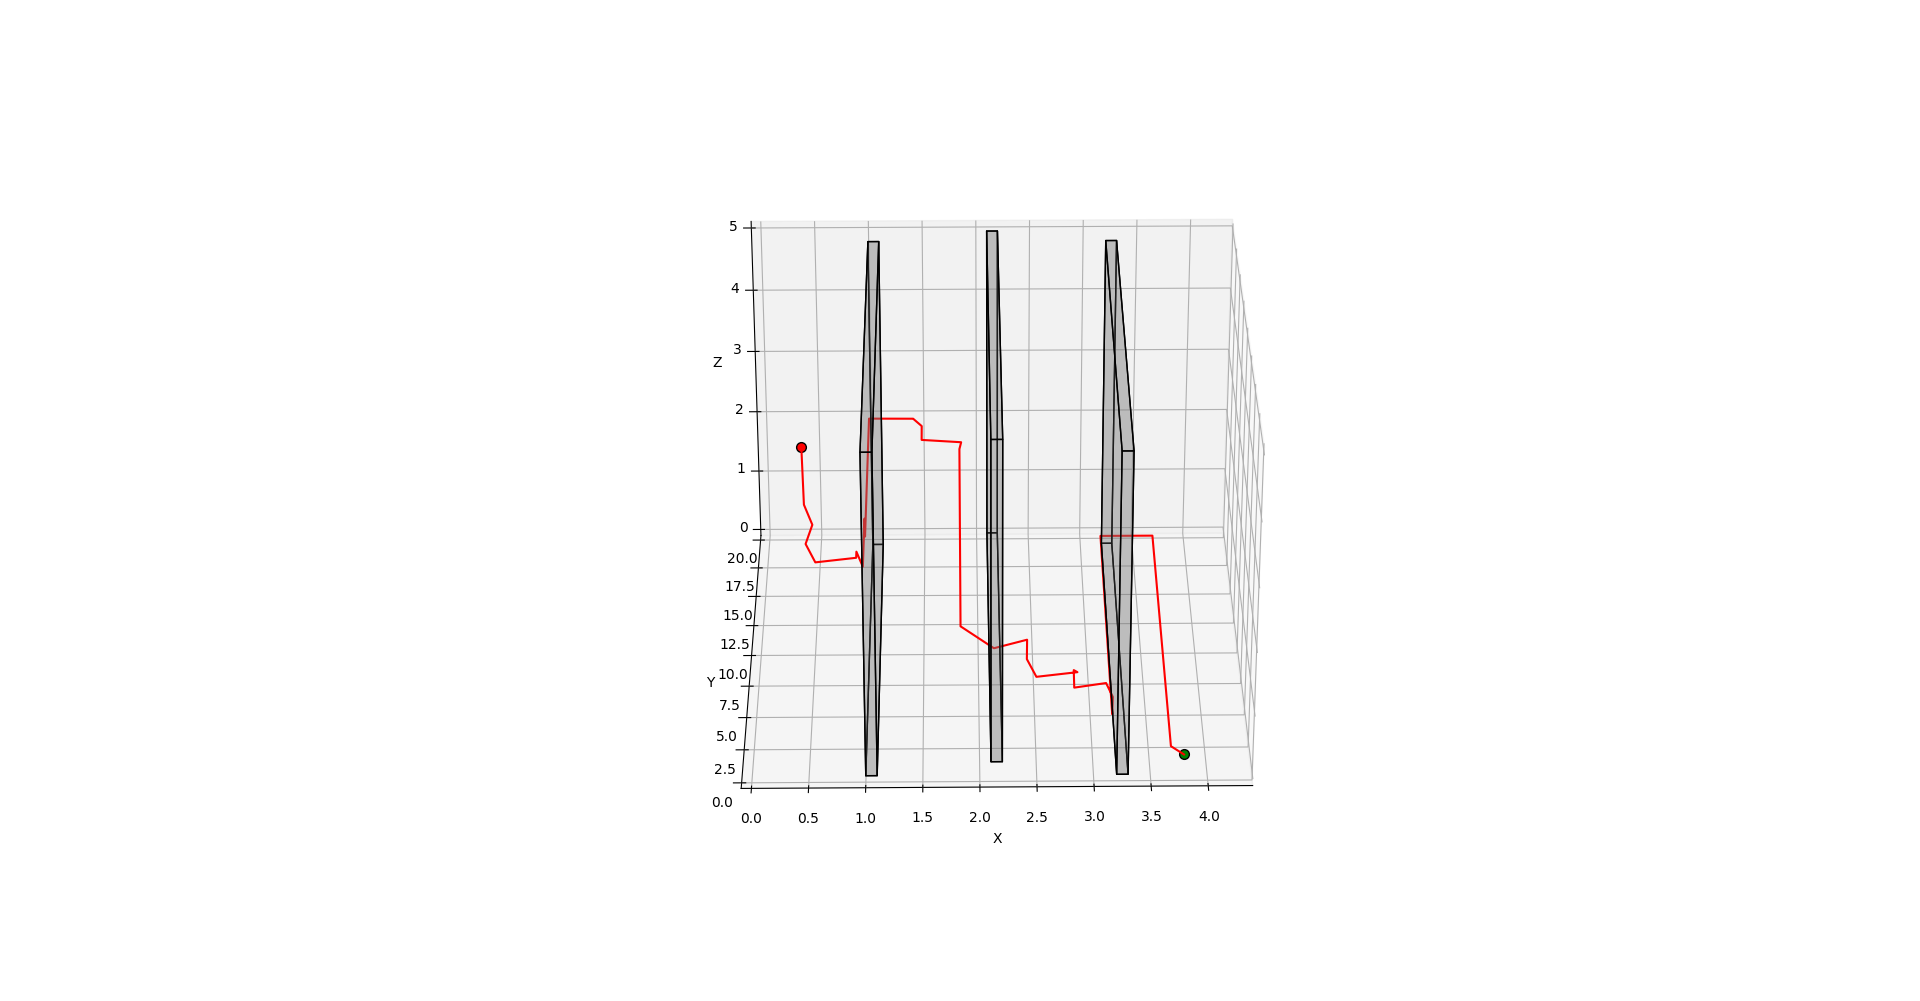
\includegraphics[width=0.6\textwidth]{monza_astar_m.png}
    \caption{Monza Environment}
    \label{fig:monza_astar_m}
\end{figure}
\begin{figure}[H]
    \centering
    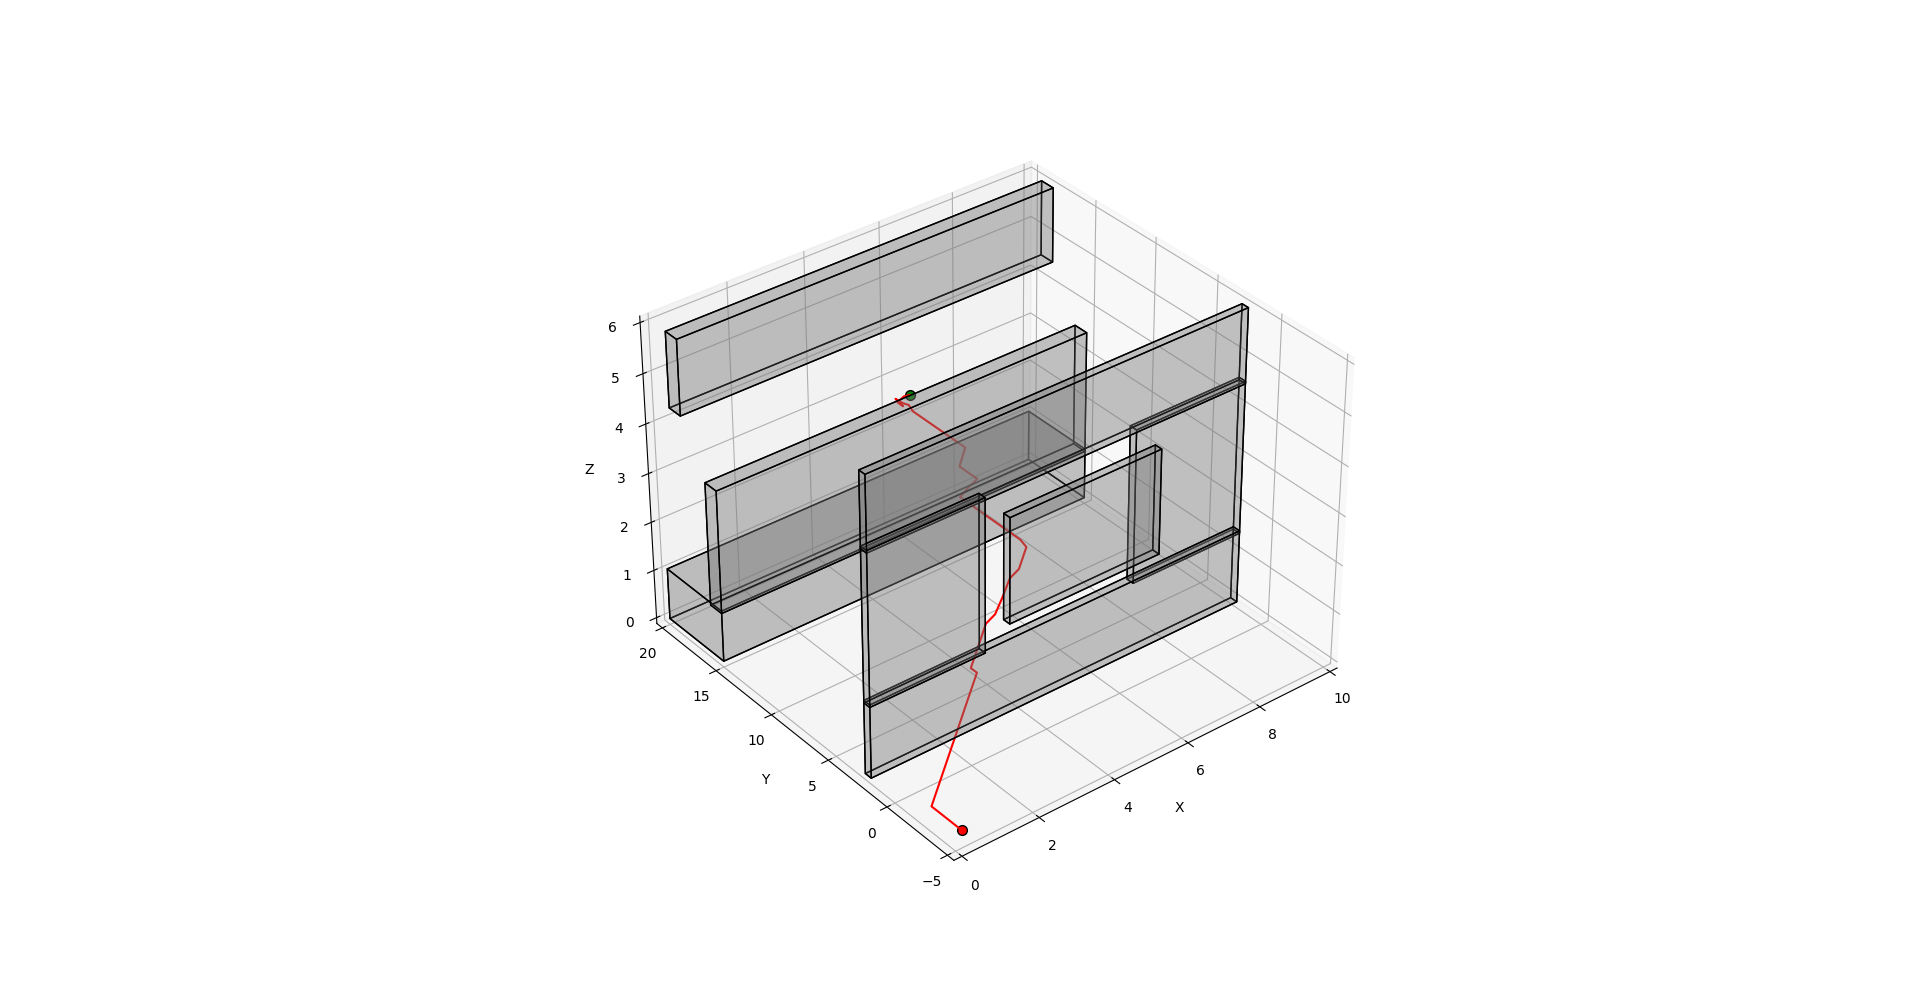
\includegraphics[width=0.6\textwidth]{window_astar_o.png}
    \caption{Window Environment}
    \label{fig:window_astar_m}
\end{figure}
\begin{figure}[H]
    \centering
    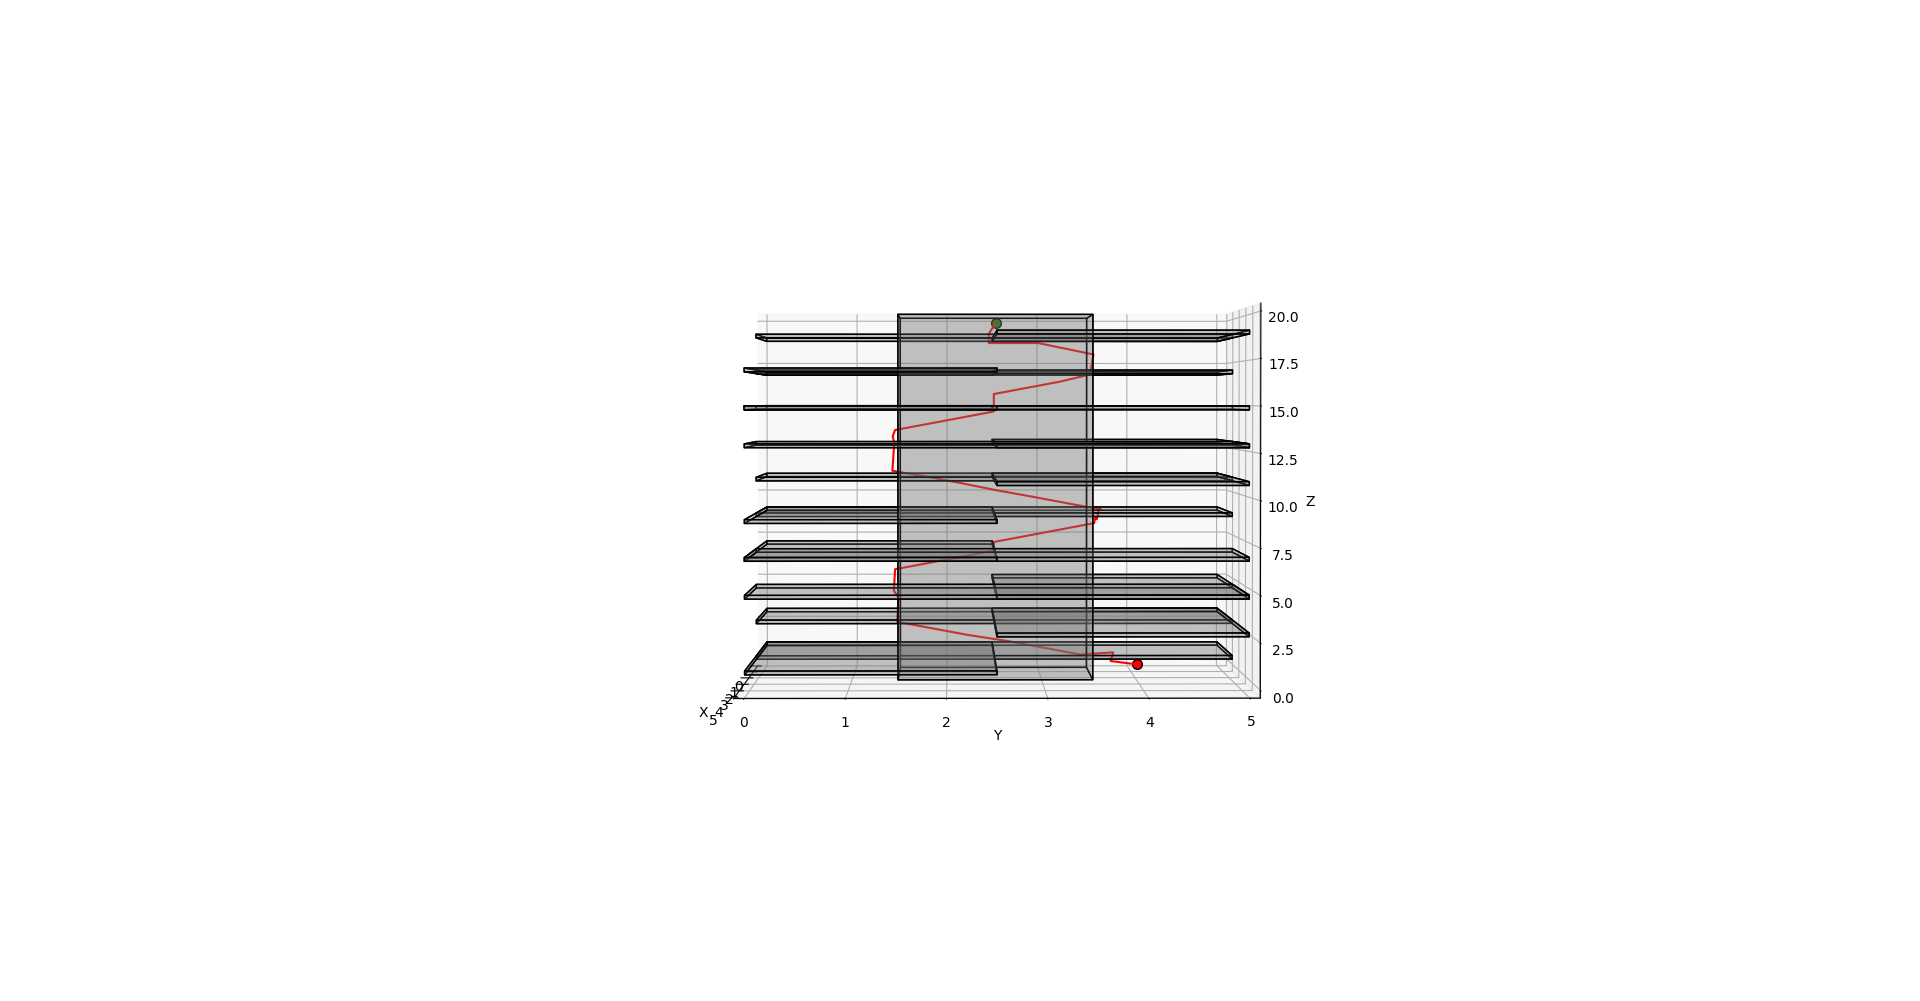
\includegraphics[width=0.6\textwidth]{tower_astar_m.png}
    \caption{Tower Environment}
    \label{fig:tower_astar_m}
\end{figure}
\begin{figure}[H]
    \centering
    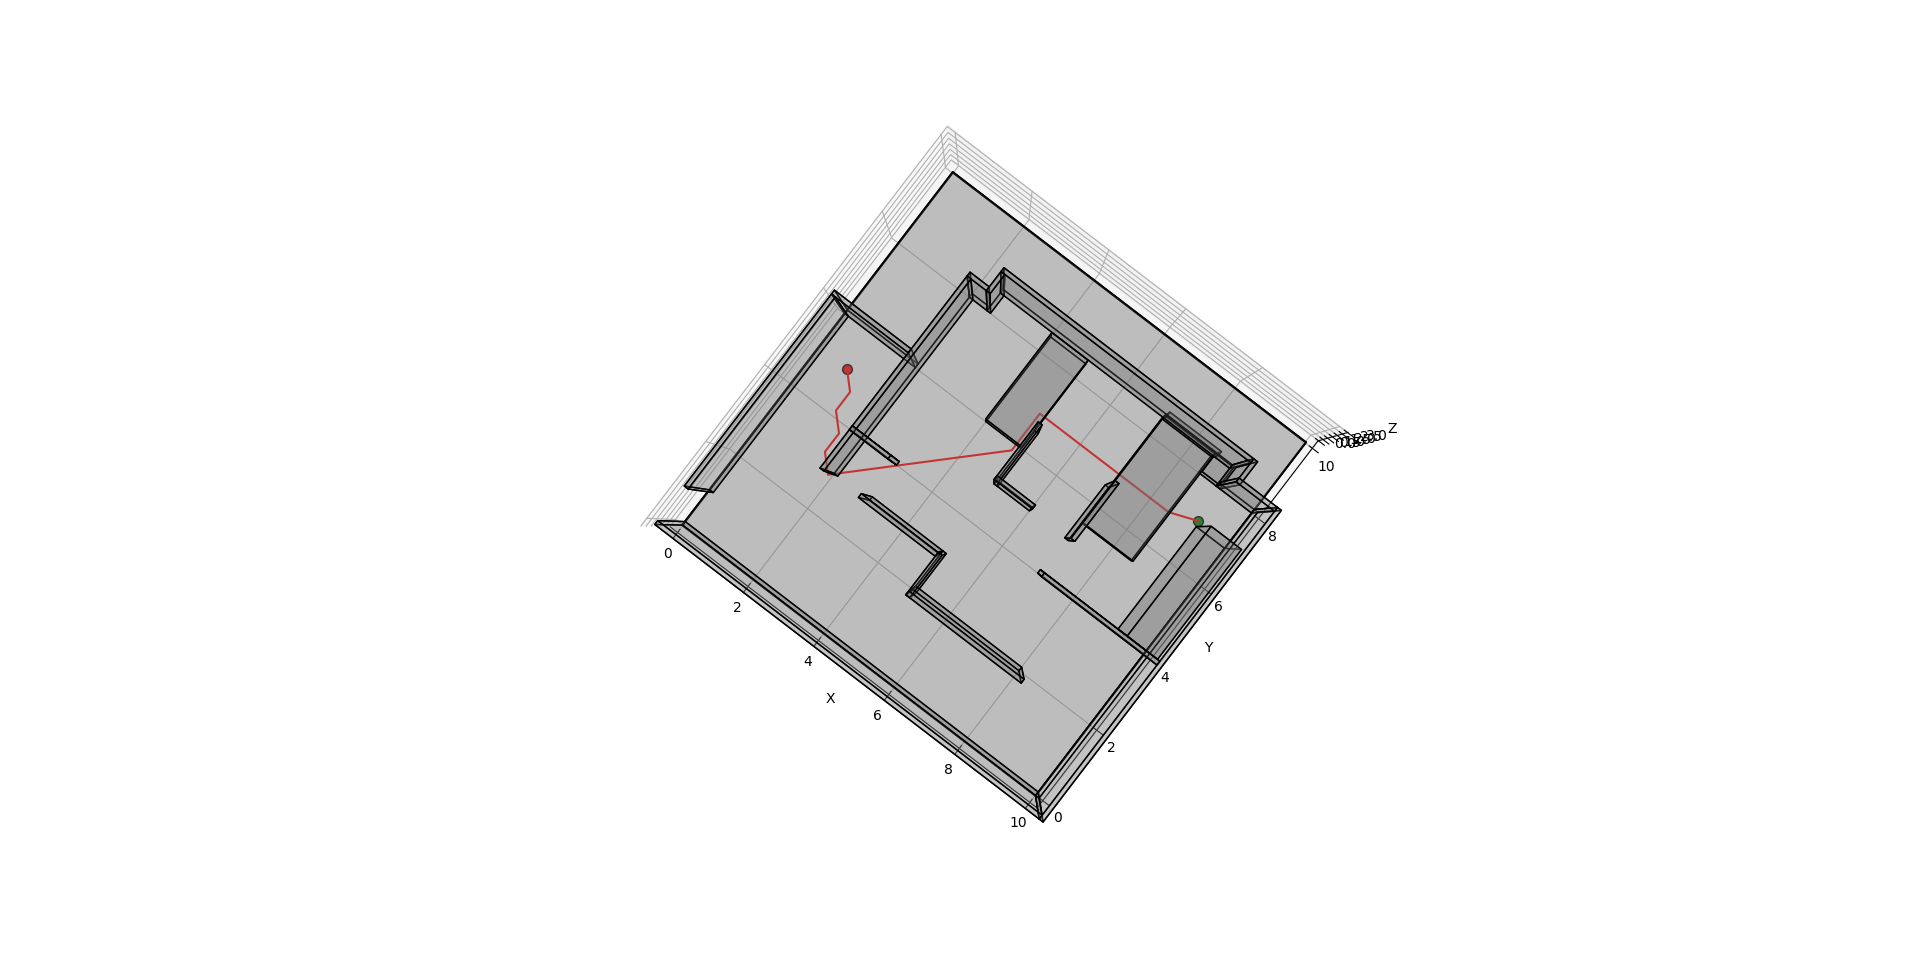
\includegraphics[width=0.6\textwidth]{room_astar_m.png}
    \caption{Room Environment}
    \label{fig:room_astar_m}
\end{figure}
\subsection{RRT with Uniform Sampling Distribution}
\begin{figure}[H]
    \centering
    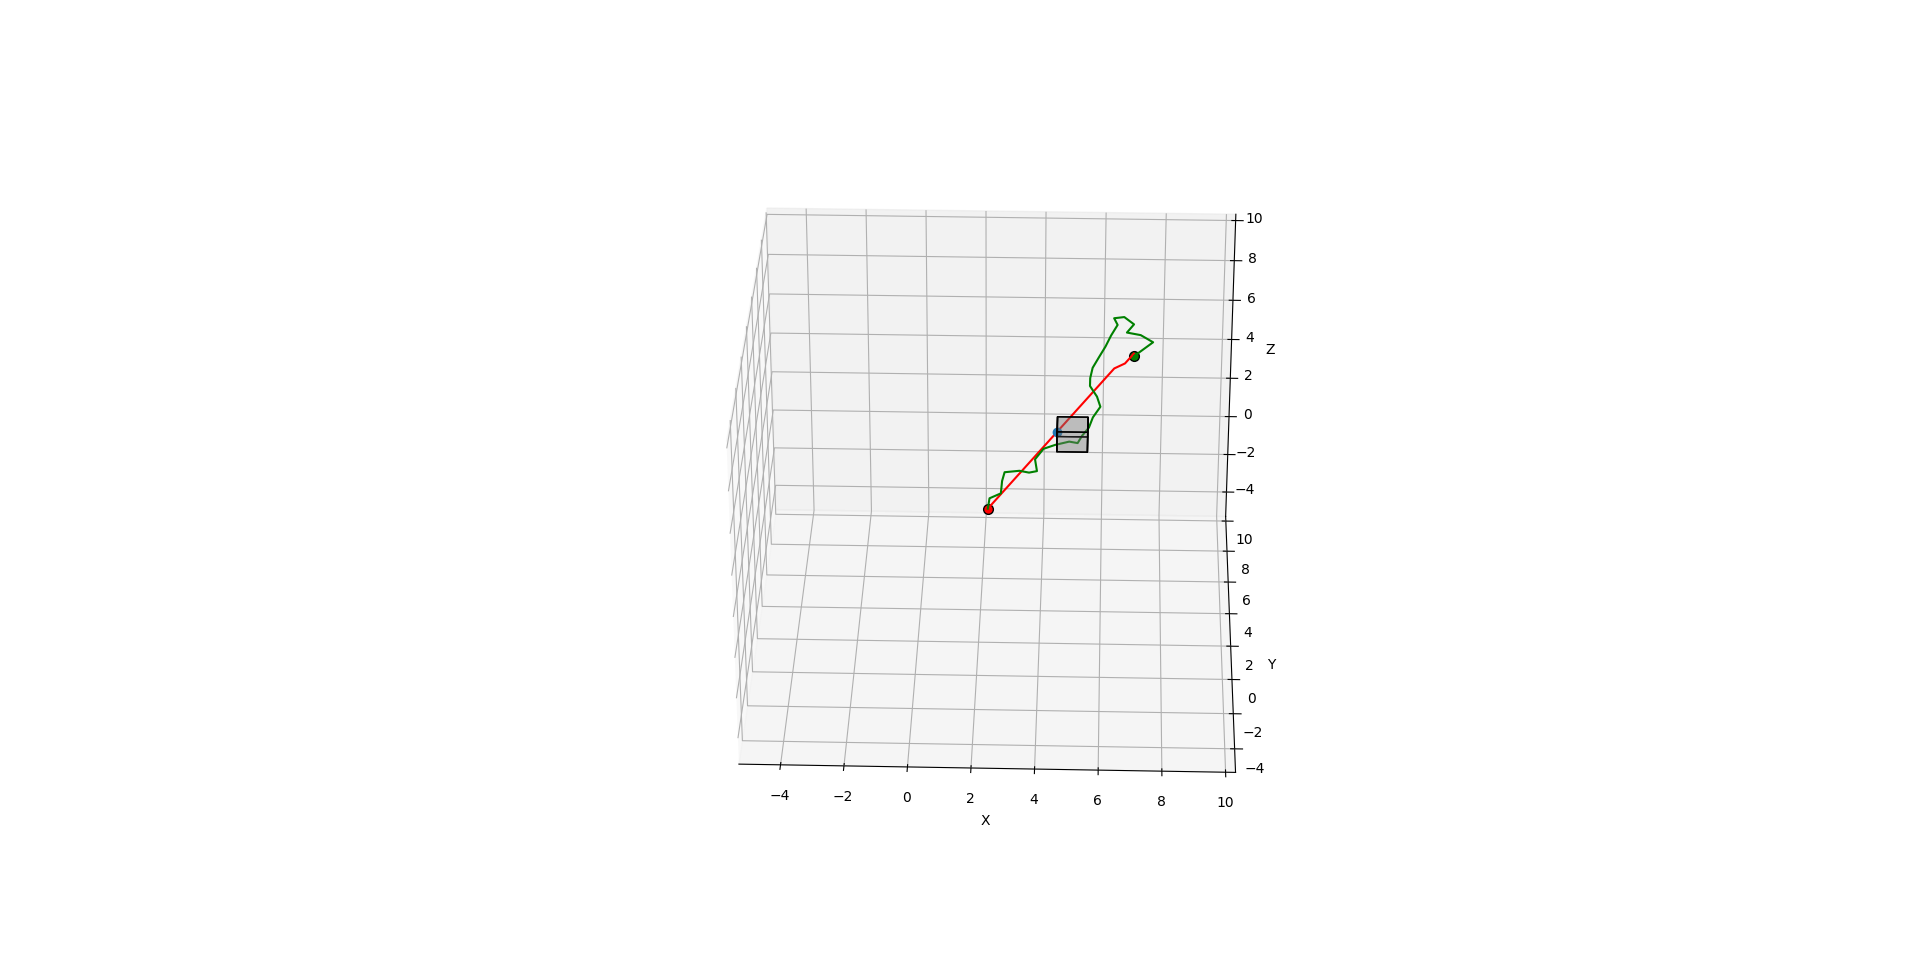
\includegraphics[width=0.6\textwidth]{cube_rrt.png}
    \caption{Single Cube Environment}
    \label{fig:cube_rrt}
\end{figure}
\begin{figure}[H]
    \centering
    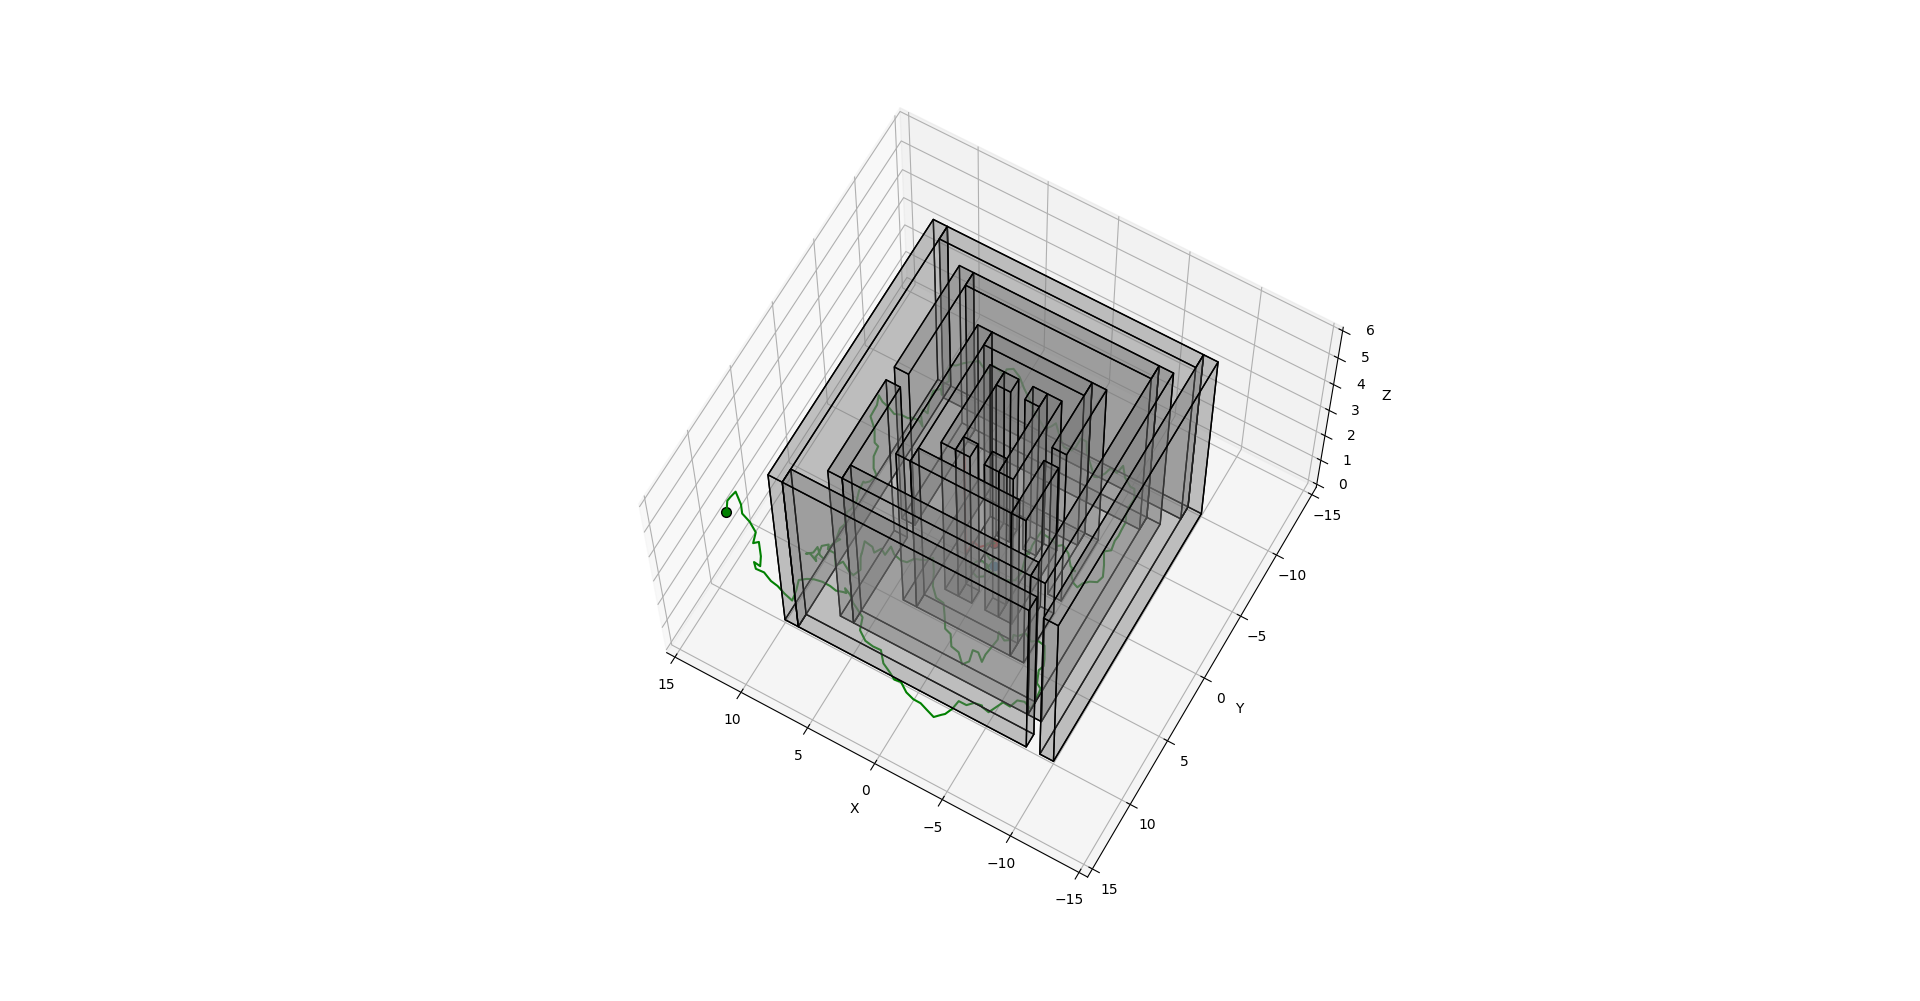
\includegraphics[width=0.6\textwidth]{maze_rrt.png}
    \caption{Maze Environment}
    \label{fig:maze_rrt}
\end{figure}
\begin{figure}[H]
    \centering
    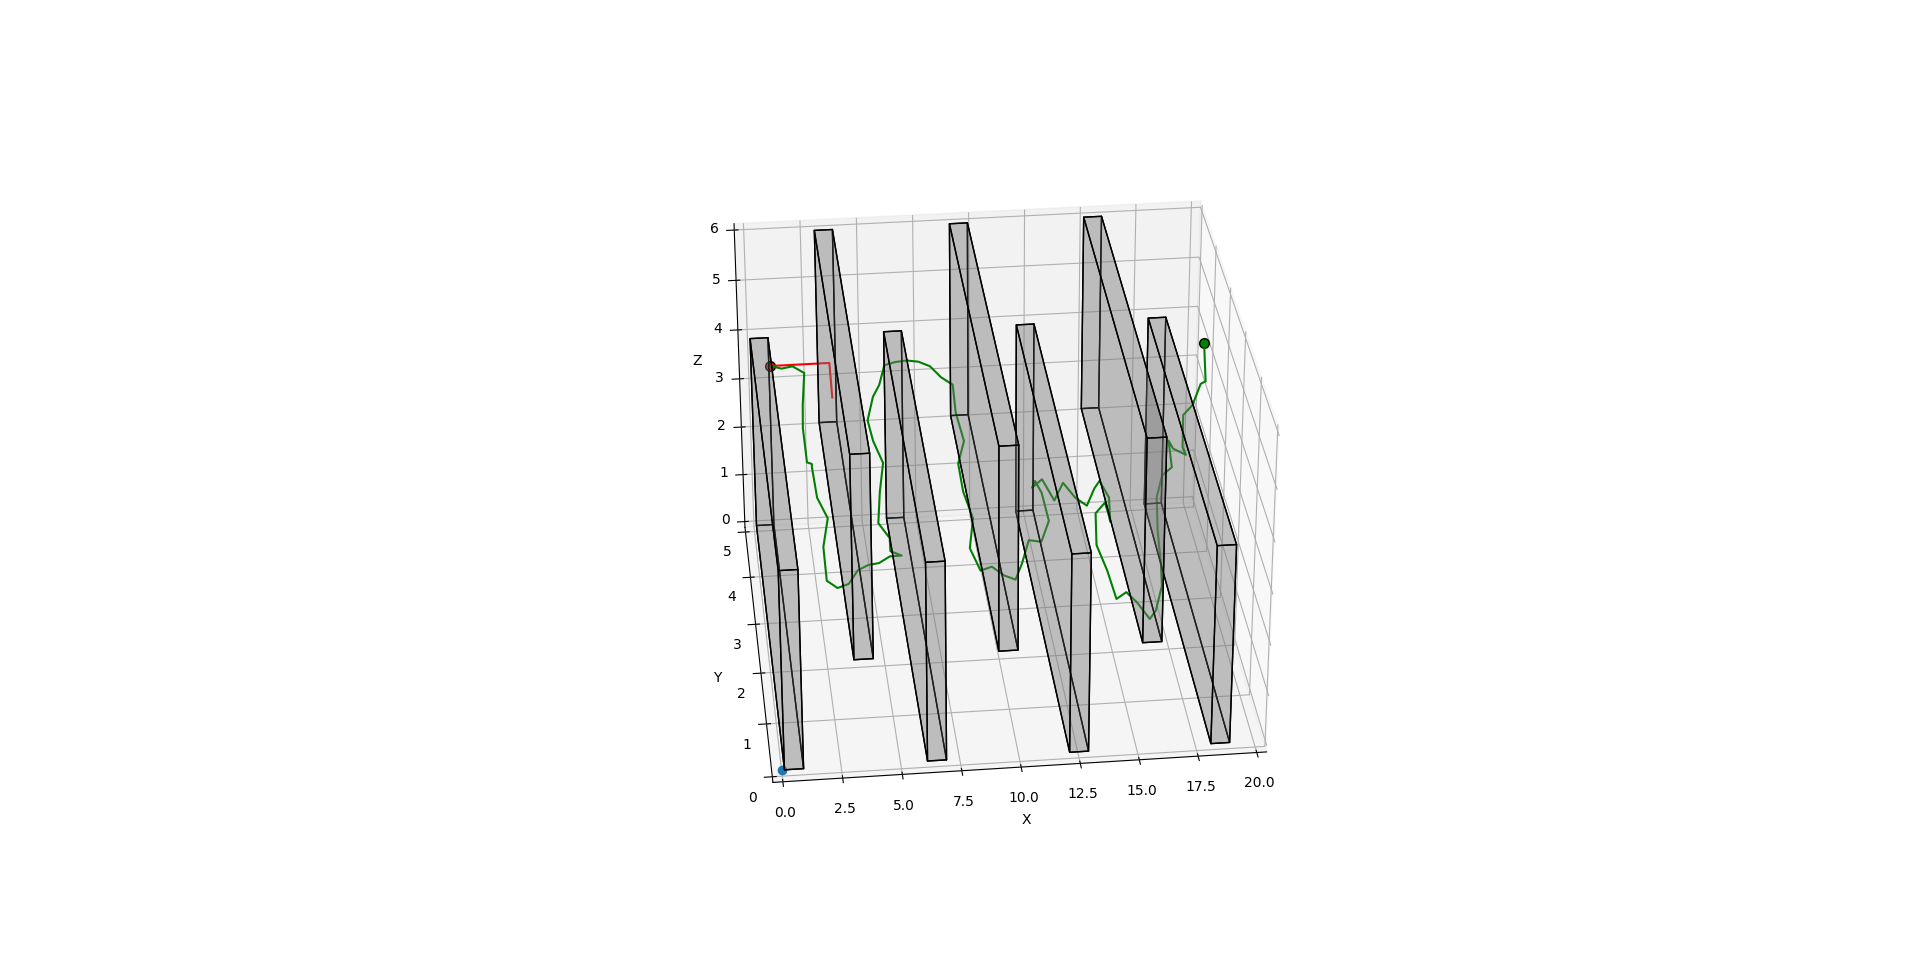
\includegraphics[width=0.6\textwidth]{flappy_bird_rrt.png}
    \caption{Flappy Bird Environment}
    \label{fig:flappy_bird_rrt}
\end{figure}
\begin{figure}[H]
    \centering
    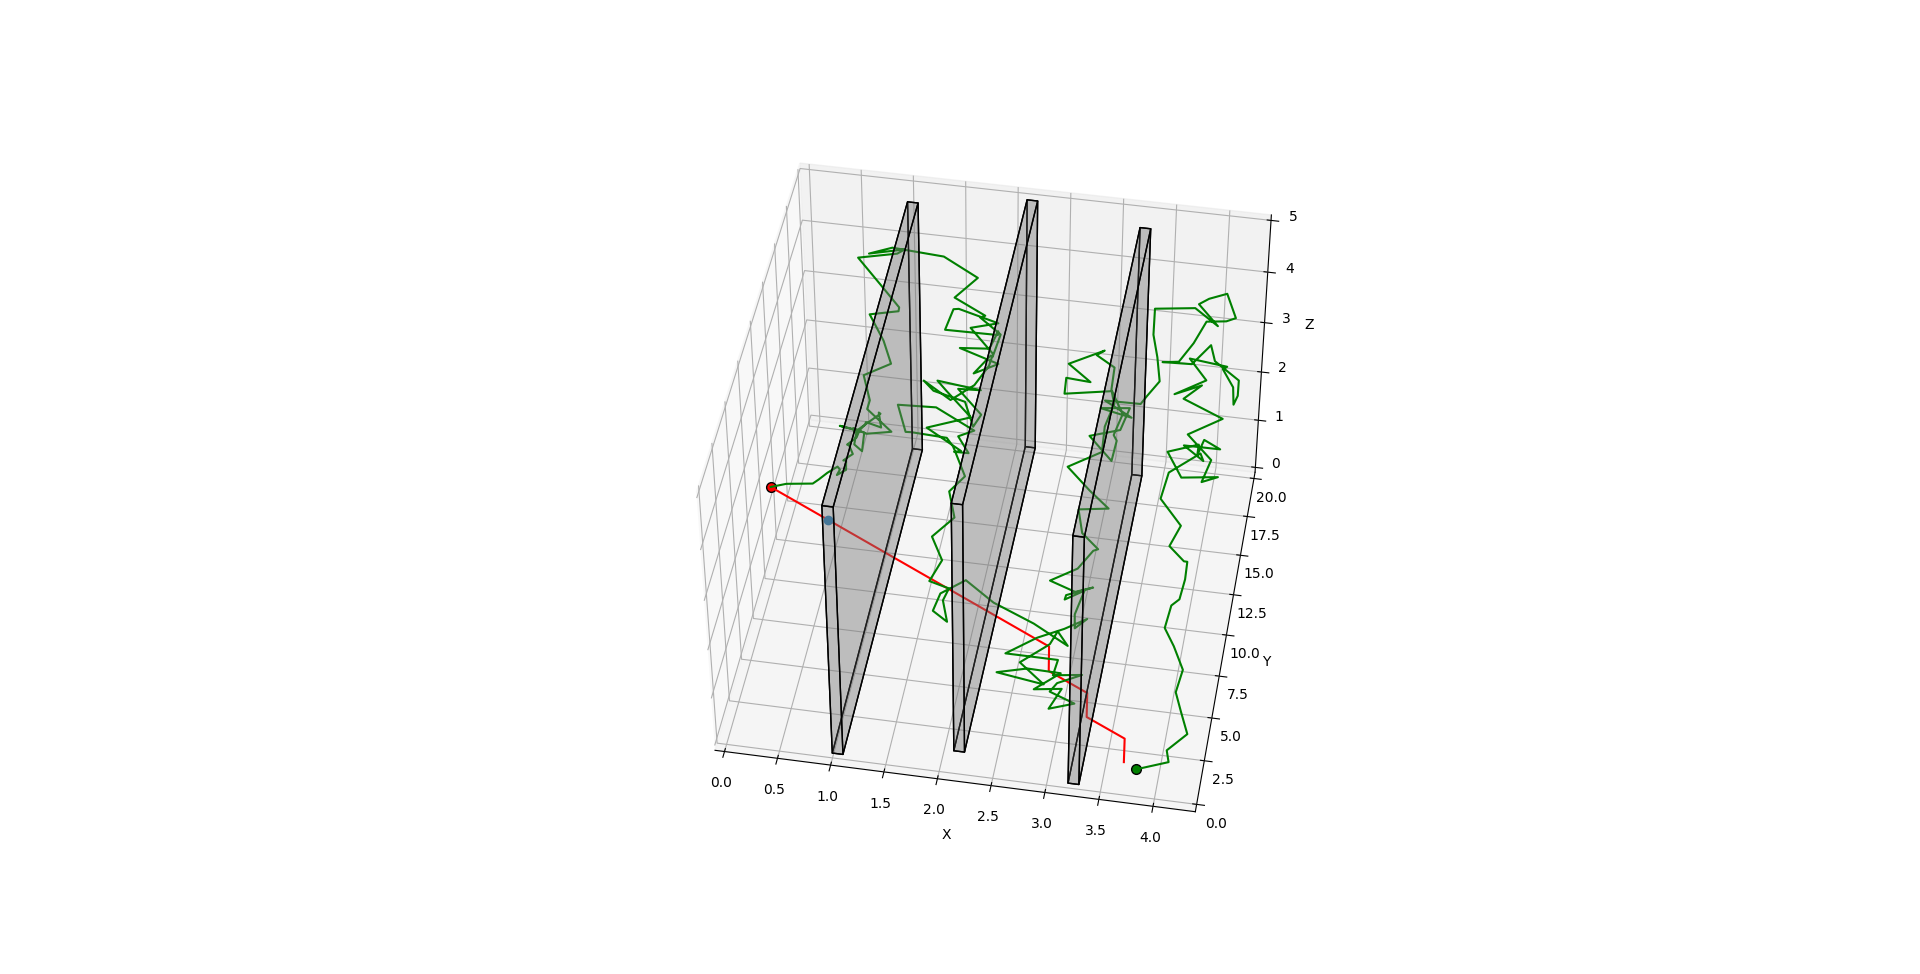
\includegraphics[width=0.6\textwidth]{monza_rrt.png}
    \caption{Monza Environment}
    \label{fig:monza_rrt}
\end{figure}
\begin{figure}[H]
    \centering
    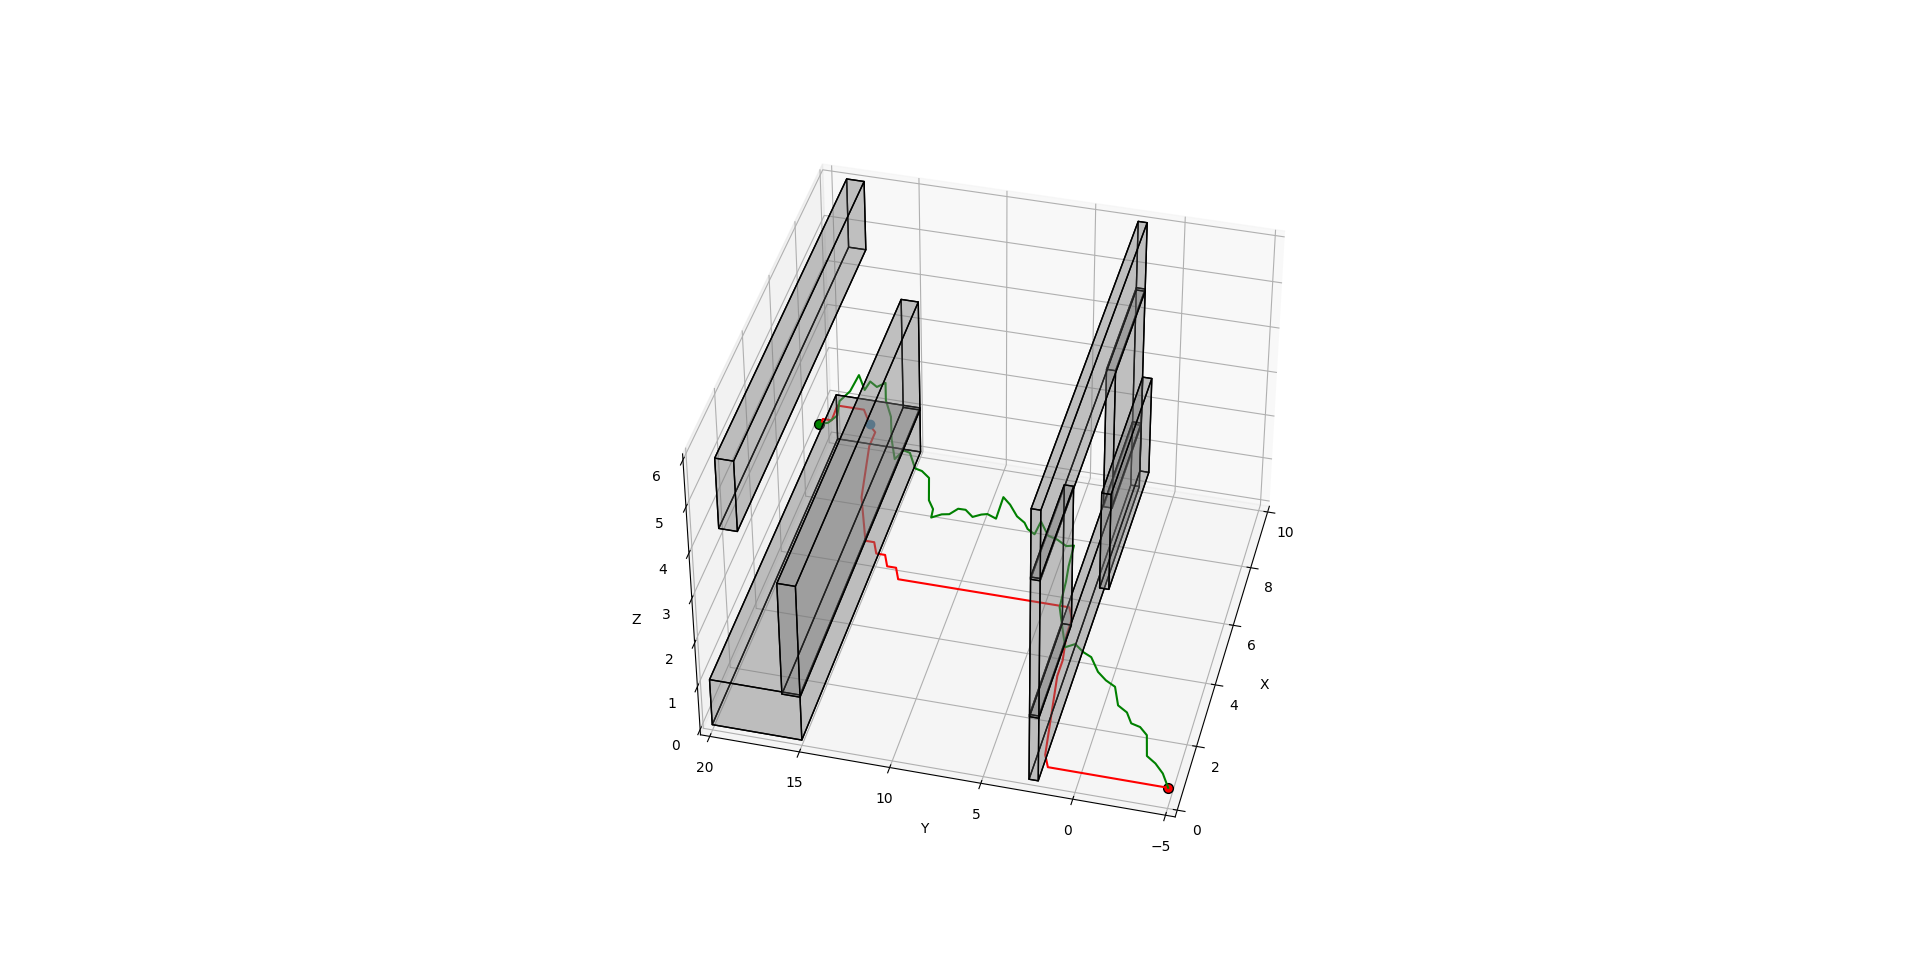
\includegraphics[width=0.6\textwidth]{window_rrt.png}
    \caption{Window Environment}
    \label{fig:window_rrt}
\end{figure}
\begin{figure}[H]
    \centering
    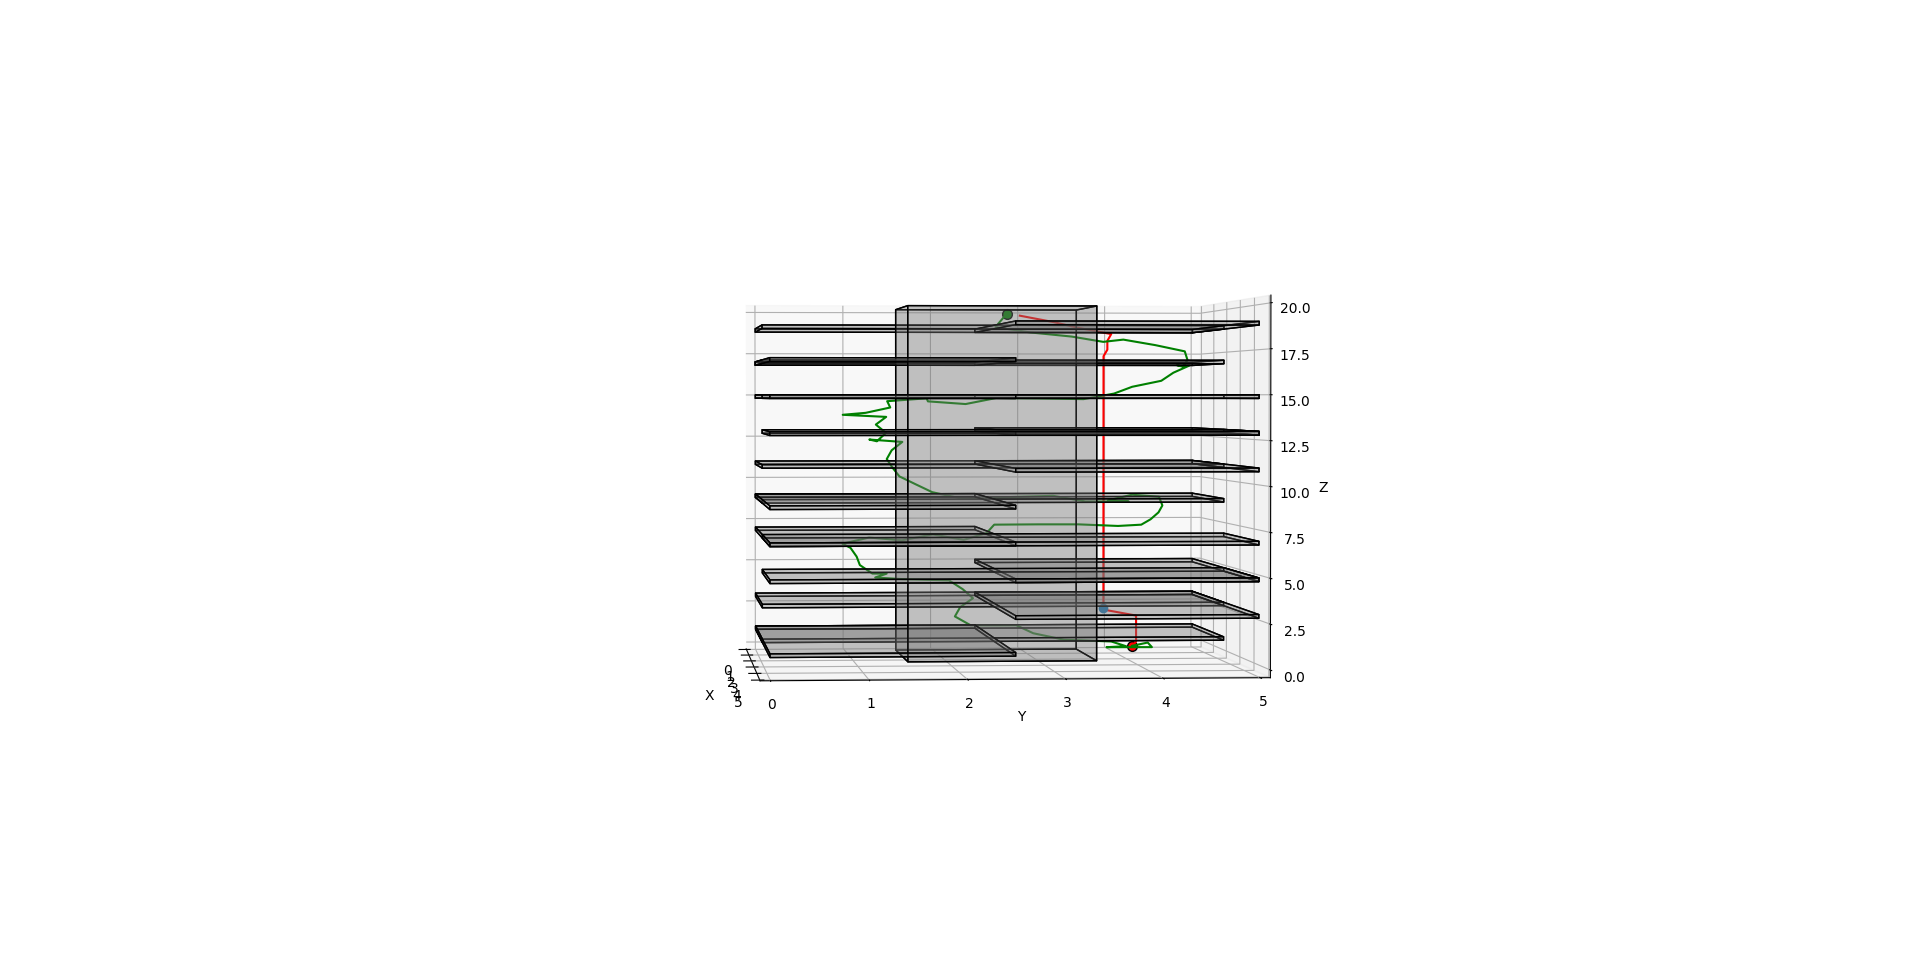
\includegraphics[width=0.6\textwidth]{tower_rrt.png}
    \caption{Tower Environment}
    \label{fig:tower_rrt}
\end{figure}
\begin{figure}[H]
    \centering
    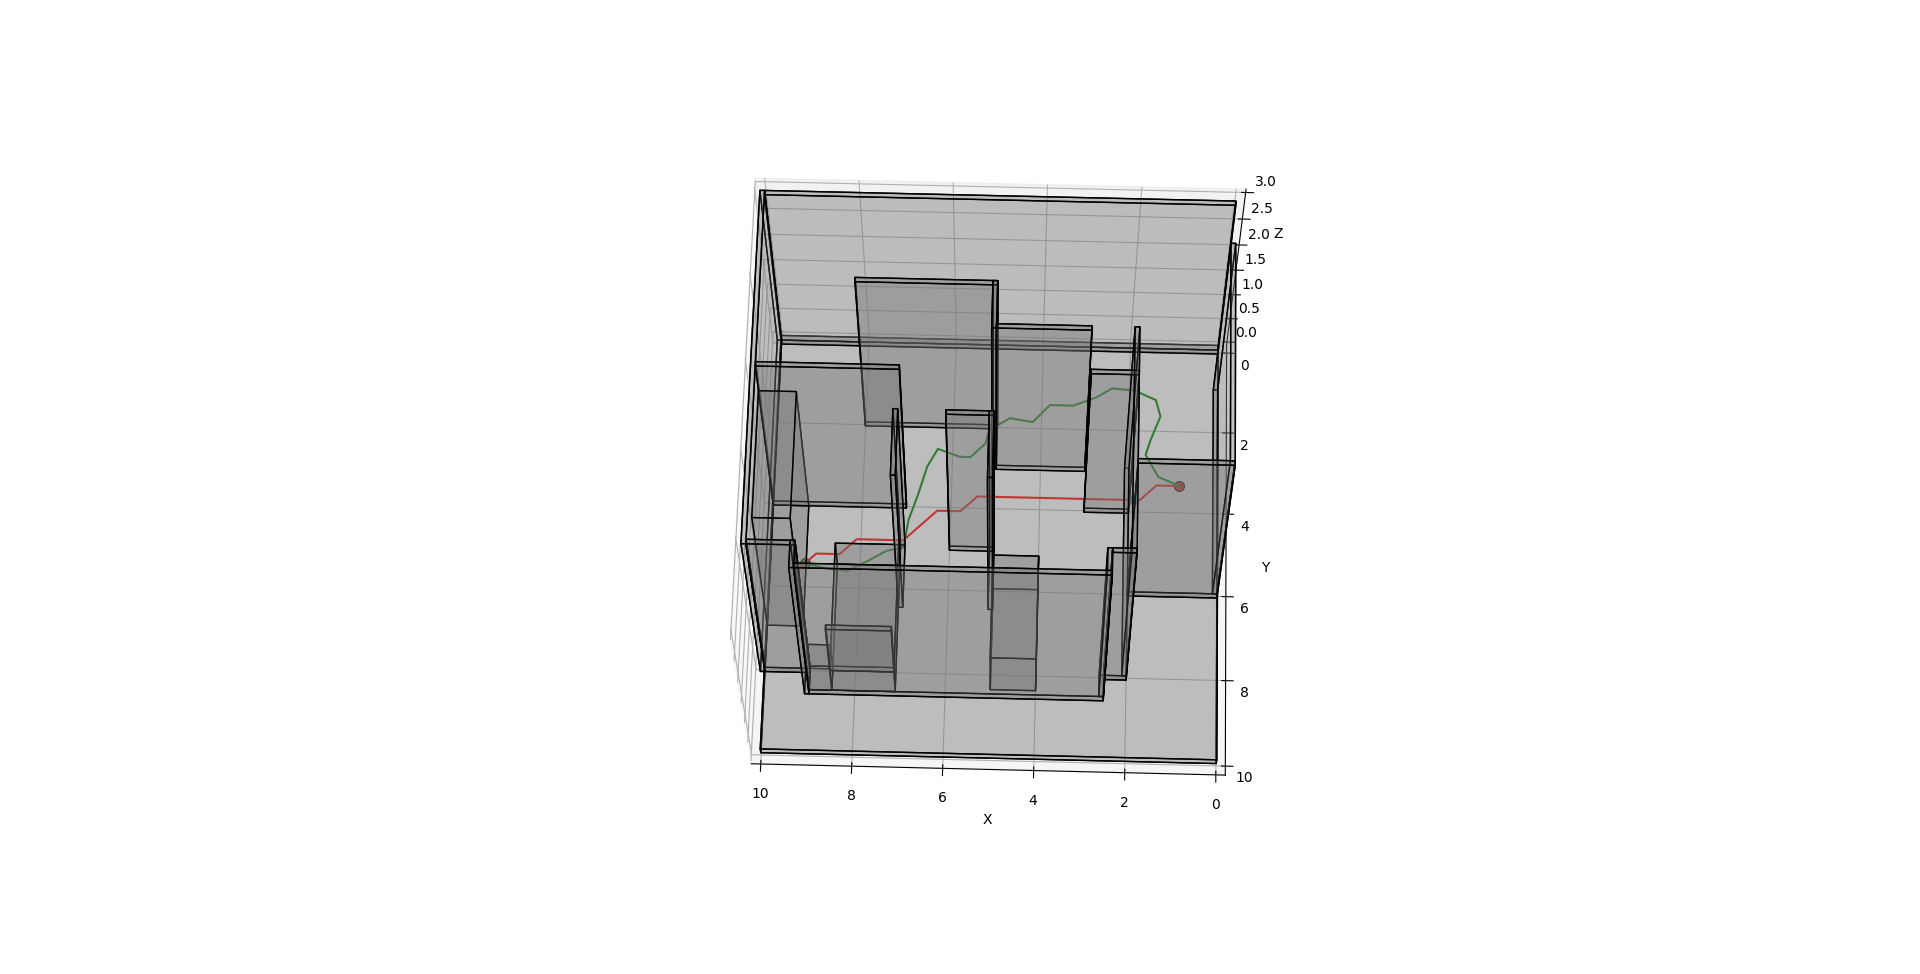
\includegraphics[width=0.6\textwidth]{room_rrt.png}
    \caption{Room Environment}
    \label{fig:room_rrt}
\end{figure}
\subsection{RRT with Biased Sampling Distribution}
\begin{figure}[H]
    \centering
    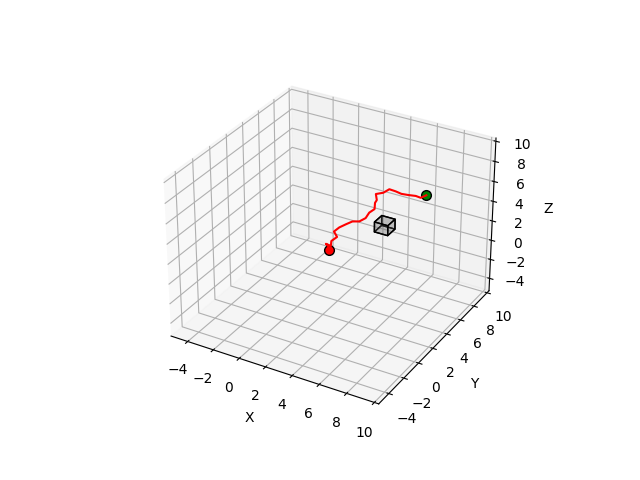
\includegraphics[width=0.6\textwidth]{cube_rrt_b.png}
    \caption{Single Cube Environment}
    \label{fig:cube_rrt_biased}
\end{figure}
\begin{figure}[H]
    \centering
    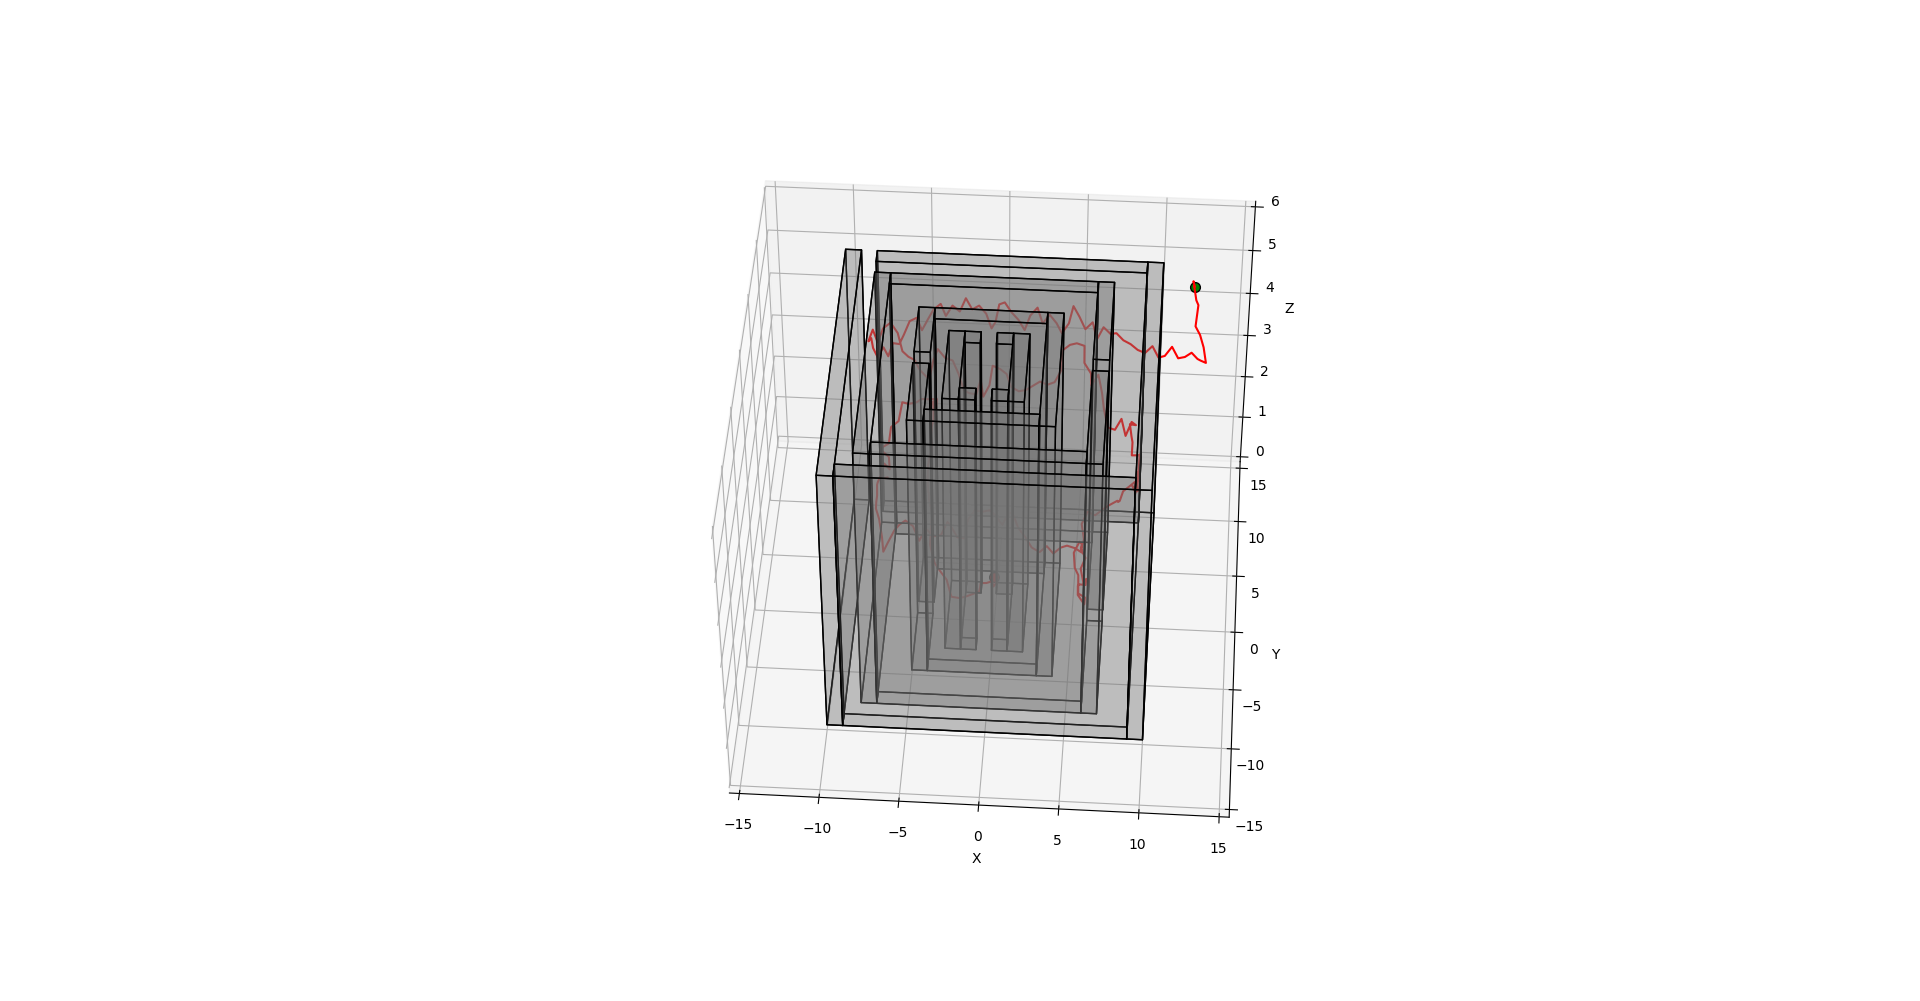
\includegraphics[width=0.6\textwidth]{maze_rrt_b.png}
    \caption{Maze Environment}
    \label{fig:maze_rrt_biased}
\end{figure}
\begin{figure}[H]
    \centering
    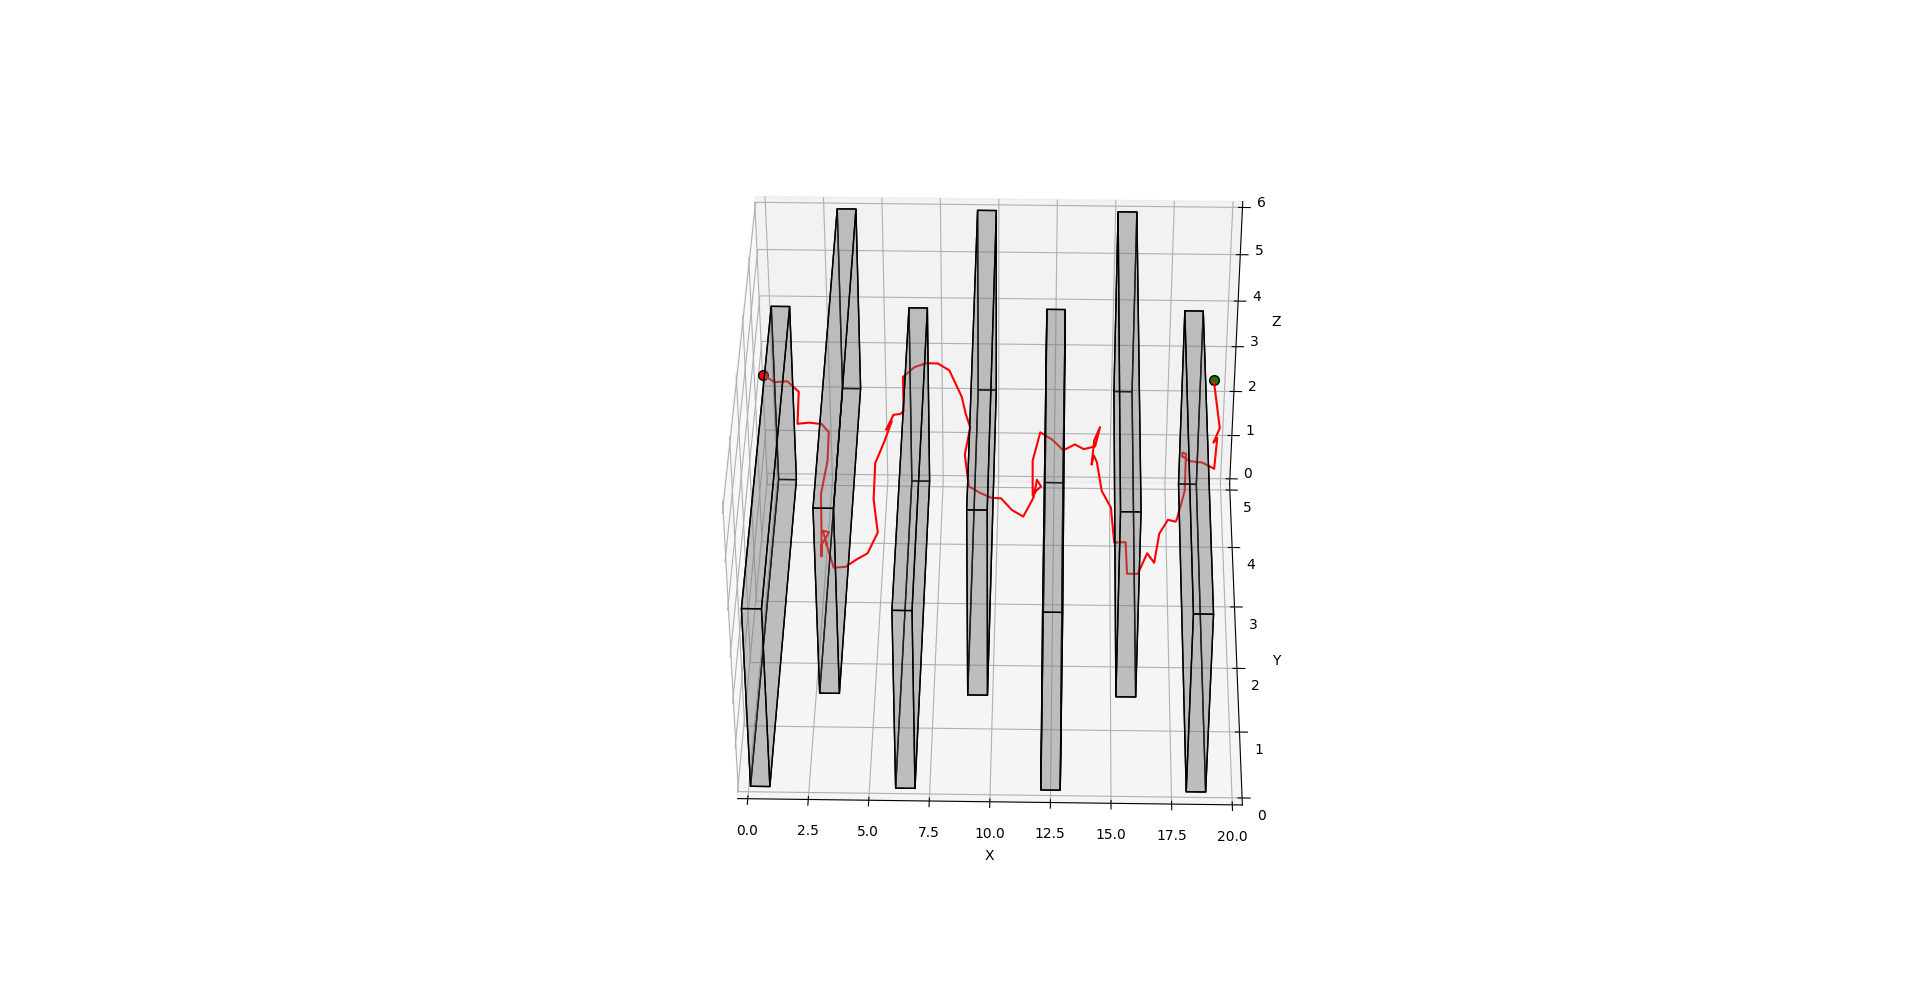
\includegraphics[width=0.6\textwidth]{flappy_bird_rrt_b.png}
    \caption{Flappy Bird Environment}
    \label{fig:flappy_bird_rrt_biased}
\end{figure}

\begin{figure}[H]
    \centering
    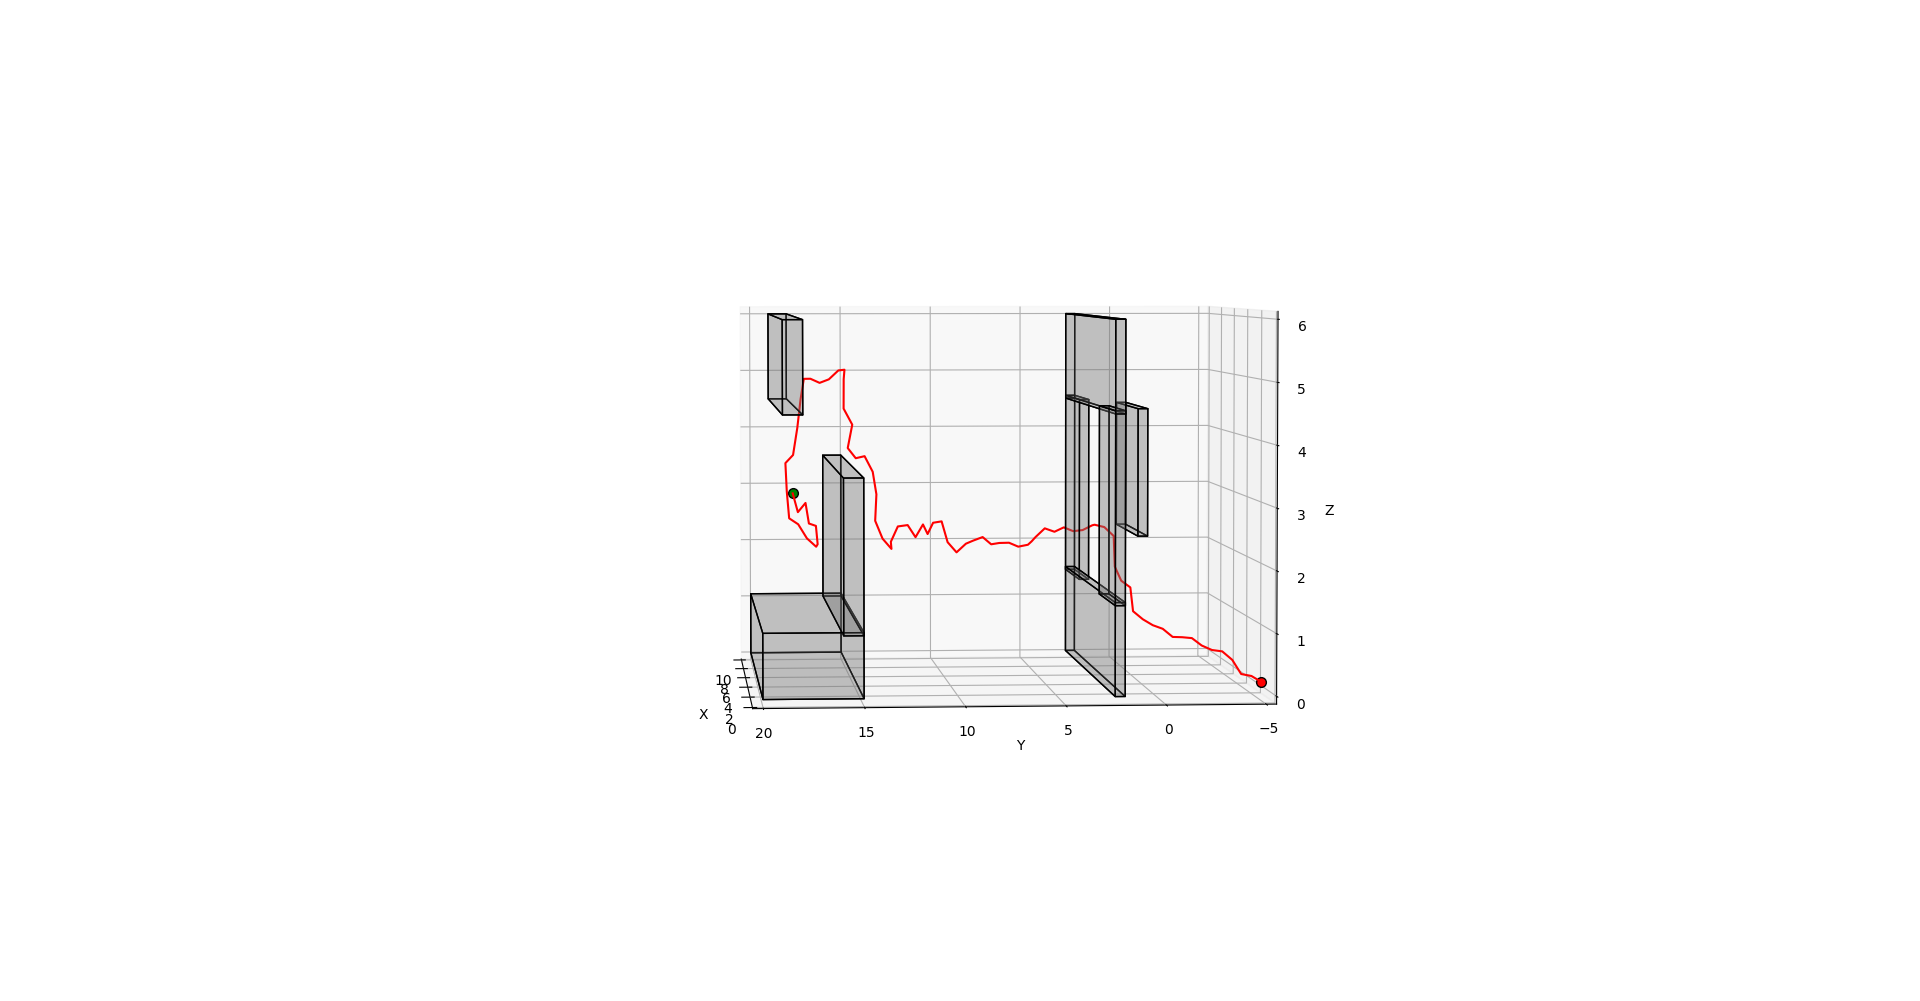
\includegraphics[width=0.6\textwidth]{window_rrt_b.png}
    \caption{Window Environment}
    \label{fig:window_rrt_biased}
\end{figure}
\begin{figure}[H]
    \centering
    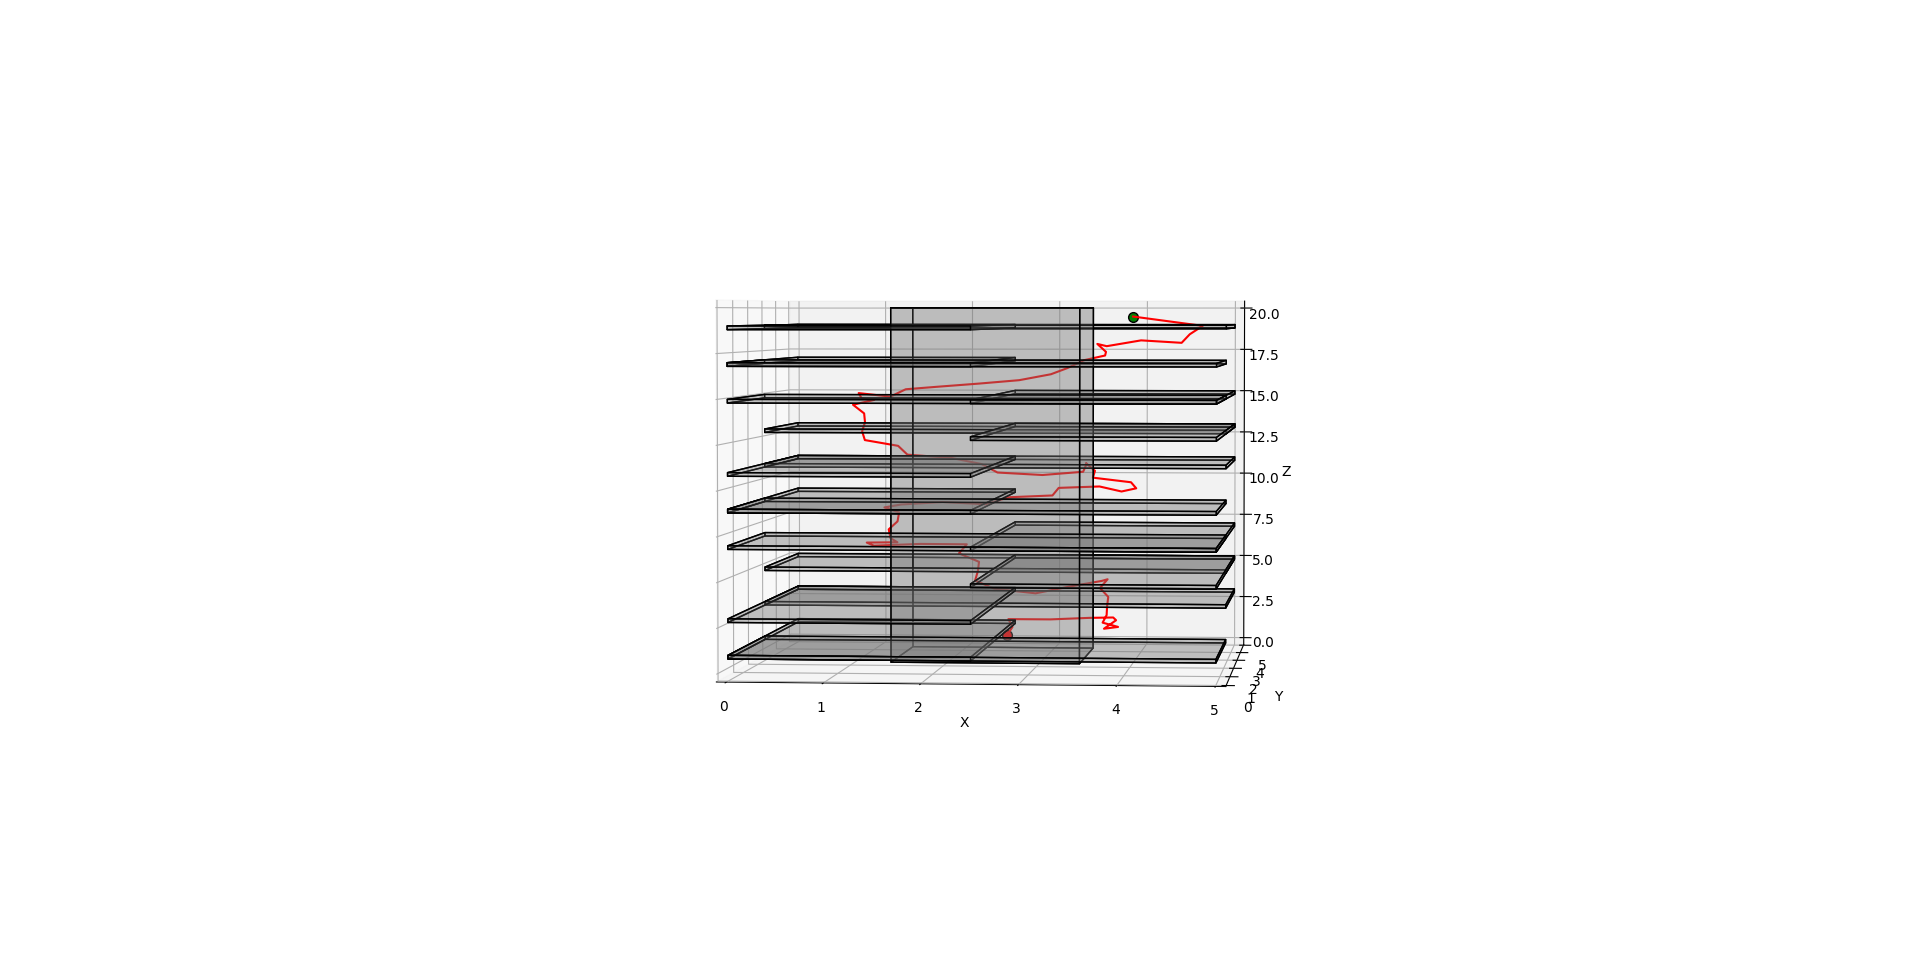
\includegraphics[width=0.6\textwidth]{tower_rrt_b.png}
    \caption{Tower Environment}
    \label{fig:tower_rrt_biased}
\end{figure}
\begin{figure}[H]
    \centering
    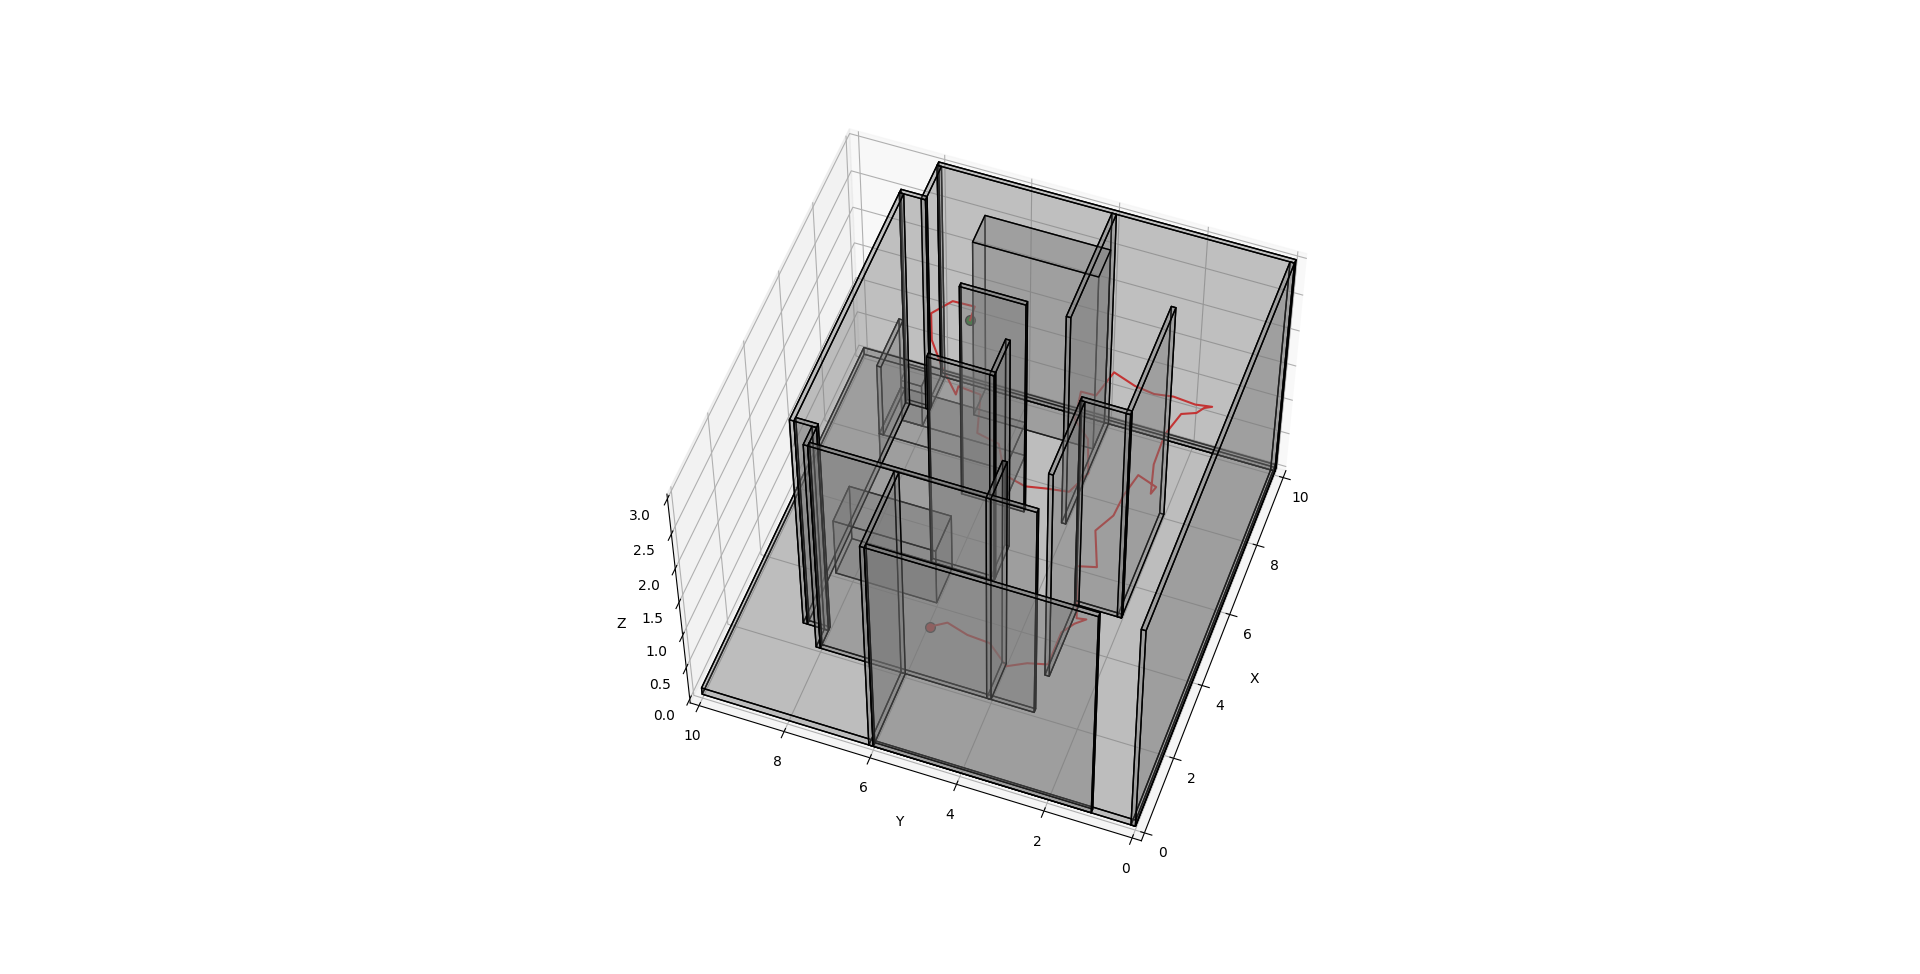
\includegraphics[width=0.6\textwidth]{room_rrt_b.png}
    \caption{Room Environment}
    \label{fig:room_rrt_biased}
\end{figure}
\begin{figure}[H]
    \centering
    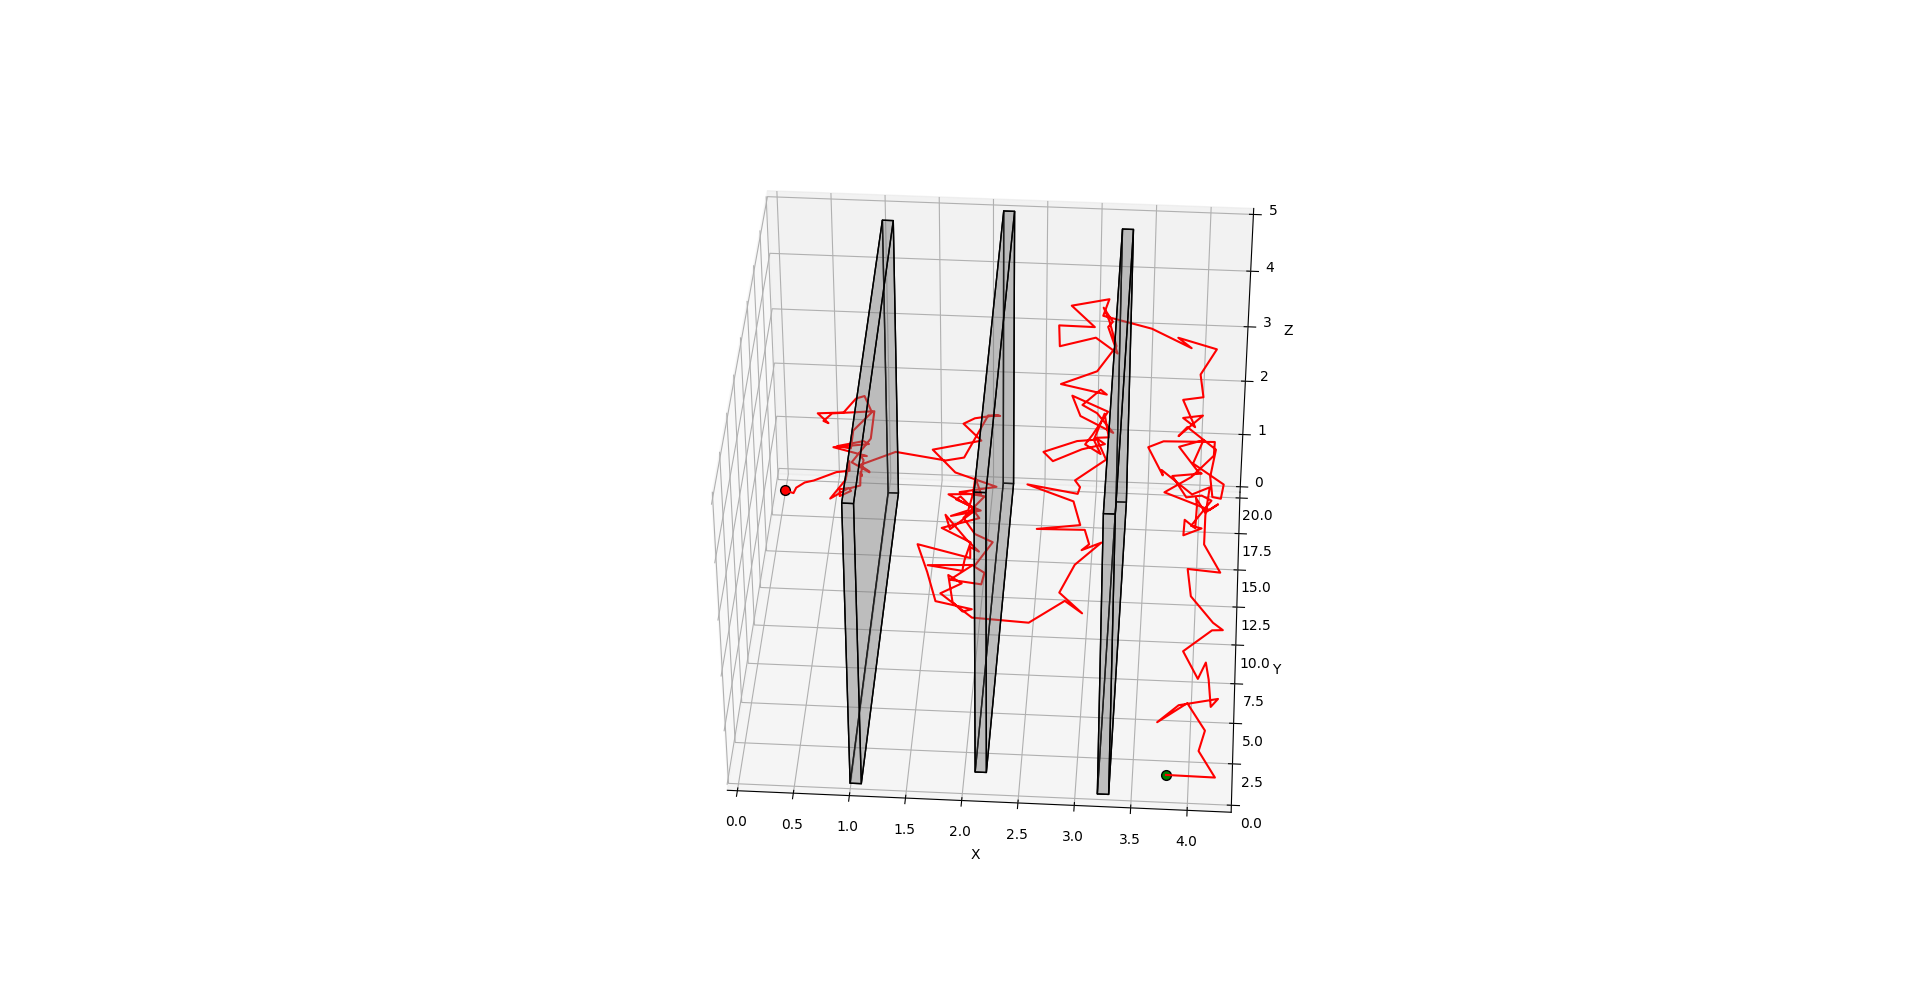
\includegraphics[width=0.6\textwidth]{monza_rrt_b.png}
    \caption{Monza Environment}
    \label{fig:monza_rrt_biased}
\end{figure}
\end{document}
